\documentclass[9pt]{beamer}
\usetheme{metropolis}

\makeatletter
\setbeamertemplate{headline}{%
  \begin{beamercolorbox}[colsep=1.5pt]{upper separation line head}
  \end{beamercolorbox}
  \begin{beamercolorbox}{section in head/foot}
    \vskip2pt\insertnavigation{\paperwidth}\vskip2pt
  \end{beamercolorbox}%
  \begin{beamercolorbox}[colsep=1.5pt]{lower separation line head}
  \end{beamercolorbox}
}
\makeatother

\setbeamercolor{section in head/foot}{fg=normal text.bg, bg=structure.fg}


\usepackage{booktabs}
\usepackage{longtable}
\usepackage{array}
\usepackage{multirow}
\usepackage{wrapfig}
\usepackage{float}
\usepackage{colortbl}
\usepackage{pdflscape}
\usepackage{tabu}
\usepackage{threeparttable}
\usepackage{threeparttablex}
\usepackage[normalem]{ulem}
\usepackage{makecell}
\usepackage{xcolor}
\usepackage[utf8]{inputenc}
\usepackage[absolute,overlay]{textpos}

\definecolor{red}{RGB}{150, 0, 0}
\definecolor{RED}{RGB}{255, 0, 0}
\definecolor{green}{RGB}{0, 85, 0}

\definecolor{GreenTOL}{HTML}{225522}
\setbeamercolor{example text}{fg=GreenTOL}
\setbeamercolor{alerted text}{fg=red}
\metroset{block=fill}
\setbeamercolor{block title alerted}{use=alerted text, fg=alerted text.fg, bg=alerted text.bg!80!alerted text.fg}
\setbeamercolor{block body alerted}{use={block title alerted, alerted text}, fg=alerted text.fg, bg=block title alerted.bg!50!alerted text.bg}
\setbeamercolor{block title example}{use=example text, fg=example text.fg, bg=example text.bg!80!example text.fg}
\setbeamercolor{block body example}{use={block title example, example text}, fg=example text.fg, bg=block title example.bg!50!example text.bg}

\title{A log-ratio approach to cluster analysis of count data when the total is irrelevant}
\date{}
\author{%
  \texorpdfstring{
    \begin{columns}%[onlytextwidth]
      \column{.35\linewidth}
      \centering
      \textbf{M. Comas-Cufí\inst{1}}\\
      \href{mailto:marc.comas@udg.edu}{marc.comas@udg.edu}\\ \vspace{0.5cm}
      \
      G. Mateu-Figueras\inst{1}\\
      \href{mailto:gloria.mateu@udg.edu}{gloria.mateu@udg.edu}\\
      \column{.35\linewidth}
      \centering
      J.A. Martín-Fernández\inst{1}\\
      \href{mailto:josepantoni.martin@udg.edu}{josepantoni.martin@udg.edu}\\   \vspace{0.5cm}
      J. Palarea-Albaladejo\inst{2}\\
      \href{mailto:javier.palarea@bioss.ac.uk}{javier.palarea@bioss.ac.uk}      
    \end{columns}
  }
  {}
}

\institute{\vspace{0.25cm}
\inst{1} Department of Computer Science, Applied Mathematics and Statistics, Universitat de Girona, Girona \\

\includegraphics[height=0.9cm]{imae.png}
\and%
\inst{2} Biomathematics and Statistics Scotland, Edinburgh\\

\includegraphics[height=1cm]{bioss.png}}

    
\begin{document}
\begin{frame}[noframenumbering]
\thispagestyle{empty}
\titlepage
\end{frame}

{
\metroset{sectionpage=none}
\section{Preliminaries}
}

\begin{frame}{Compositional data analysis}

\begin{itemize}
\item
  \textbf{Compositional data} (CoDa), \((p_1, \dots, p_{{D}})\), are
  quantitative descriptions of the parts of some whole, conveying
  \textbf{relative information}. CoDa are commonly expressed in
  proportions, percentages, or ppm  (Aitchison, 1986).
\item
The simplex
\[
S^{{D}} = \left\{ \left(p_1,\dots,p_{{D}}\right) | \; p_i > 0, \sum_{i=1}^{{D}} p_i = \kappa \right\},
\] is the sample space of CoDa.
\item
  \textbf{Log-ratios} of parts handle relative information and satisfy desirable properties such as scale invariance and subcompositional coherence: \[
  \log\left(\frac{p_i}{p_j}\right), \log\left(\frac{p_j}{\sqrt[{D}]{\prod_{\ell=1}^{{D}}p_{\ell}}} \right), \sqrt{\frac{j}{j+1}}\, \log\frac{\sqrt[j]{\prod_{\ell=1}^{j} p_\ell}}{p_{j+1}}, \dots
  \]
\end{itemize}

\end{frame}

\begin{frame}{CoDa and the zero problem}

\begin{itemize}
\item Zeros prevent from using log-ratios. Most proposals have been focused on the continuous case (\textbf{zCompositions} R package; Palarea-Albaladejo \& Martín-Fernández, 2015).
\item
  \textbf{Compositional count data sets:} discrete vectors of number of outcomes falling into mutually exclusive categories.
\begin{table}[ht]
\centering
\scriptsize
\begin{tabular}{lrrrrrrrrrr}
  \hline
\textbf{Municipality} & \textbf{jxsi} & \textbf{psc} & \textbf{pp} & \textbf{catsp} & \textbf{cs} & \textbf{cup}  \\ 
  \hline
   S. Jaume de F. &  14 &   1 &   {\color{red}0} &   2 &   {\color{red}0} &   5  \\ 
  Gisclareny &  20 &   {\color{red}0} &   {\color{red}0} &   {\color{red}0} &   1 &   2  \\ 
\vdots &  \vdots &  \vdots & \vdots & \vdots  &  \vdots & \vdots  \\
L'Hosp. de Llob. & 23843 & 28947 & 14336 & 16855 & 29773 & 7528\\
Barcelona & 326376 & 100806 & 80529 & 85841 & 155361 & 87774 \\
\end{tabular}
\end{table}
\item \textbf{Assumption 1:} The relative information is relevant, the total is not.  
\item \textbf{Assumption 2:} The probability of a part different of zero is not zero. Count zeros due to sampling limitations.

\end{itemize}

\end{frame}

\begin{frame}{Parametric approaches to cluster compositional count data set (1)}

Two sources of variability are considered: 
\begin{center}Count (observations) $\;\;\;\;\;$ Compositional (probabilities)\end{center}

\begin{itemize}
\item \textbf{{\color{red}Compositional} and {\color{red}count} variability not taken into account}. Classical methods applied to observed counts (p.e. Gaussian mixtures with the counts). \vspace{0.3cm}
\item \textbf{{\color{green}Count} variability taken into account, but not {\color{red}compositional} variability}. Mixtures of multinomial distributions.\vspace{0.3cm}
\item \textbf{{\color{green}Compositional} variability taken into account, but not {\color{red}count} variability}. Zero multiplicative replacement methods.
\begin{itemize}
\item Dirichlet prior  (Martín-Fernández \textit{et al.}, 2015)
\item Log-ratio normal  prior (Comas-Cufí \textit{et al.}, 2019)
\end{itemize}
\end{itemize}

\end{frame}

\begin{frame}{Parametric approaches to cluster compositional count data set (2)}


\begin{itemize}
\item \textbf{{\color{green}Compositional} and {\color{green}count} variability taken into account}.\vspace{0.25cm}
\begin{itemize}
\item \textit{Topic models}. Mixture of multinomials where mixing proportions are modelled in the Simplex.\vspace{0.25cm}
\begin{itemize}
\item Latent Dirichlet Allocations (Blei \textit{et al.} 2003)
\item Correlated Topic Models (Blei \& Lafferty, 2007)
\end{itemize}\vspace{0.25cm}
\item \textit{Mixtures of compounding distributions}.\vspace{0.25cm}
\begin{itemize}
\item Mixtures of Dirichlet-multinomial distributions (Holmes et al., 2012)
\item Mixtures of log-ratio-normal-multinomial distributions (Comas-Cufí et al., 2017)
\end{itemize}
\end{itemize}
\end{itemize}

\pause
\begin{alertblock}{Main limitations}
\begin{itemize}
\item Dirichlet-based approaches have  \textbf{modelling difficulties}.
\item Gaussian-based approaches have  \textbf{estimation difficulties}.
\end{itemize}
\end{alertblock}

\end{frame}

\section{Our proposal}

\begin{frame}{Classical clustering approaches applied to cluster count data}

\begin{enumerate}
\item \textbf{Dealing with zeros}. 
\begin{itemize}
\item Dirichlet-multinomial (DM) distribution: conservative in keeping the covariance structure observed in the original count data set. The regression toward the mean is moderate.
\item Zero replacement: conservative in keeping covariance structure observed in the count data set. Counts with small parts tend to define clusters by themselves.
\end{itemize}
\item \textbf{Compositional variability}. Model your data using a generic distribution defined on the Simplex. Gaussian mixtures  are easy to estimate.
\item \textbf{Count variability}. Create $B$ new samples using the posterior distribution, and find clusters using classical methods on its log-ratio coordinates.
\item \textbf{Consensus clustering}. Use a clustering ensemble method to build a final cluster  (e.g. majority voting (Dudoit \& Fridlyand, 2003)).
\end{enumerate}
\end{frame}

\section{Example: 2017 Catalan regional election}

\begin{frame}{Multivariate count data set}

\begin{itemize}
\item 947 municipalities. To illustrate the approach we only consider three parts obtained with the following amalgamations.
\begin{itemize}
\item \textbf{Pro-independence parties (ind)}: CUP (cup), Esquerra Repúblicana de Catalunya (erc), Junts per Catalunya (jxcat).
\item \textbf{Anti-independence parties (esp)}: Ciutadans (cs), Partit Popular (pp), Partit Socialista de Catalunya (psc).
\item \textbf{Mixed opinions (other)}: Catalunya si que es pot (catsp), others (other).
\end{itemize}

\end{itemize}

\only<1>{\begin{table}[H]
\centering\begingroup\fontsize{7}{9}\selectfont

\begin{tabular}{lrrrrrrrrlrrrrrrrrlrrrrrrrrlrrrrrrrrlrrrrrrrrlrrrrrrrrlrrrrrrrrlrrrrrrrrlrrrrrrrr}
\toprule
mun & catsp & cs & cup & erc & jxcat & other & pp & psc\\
\midrule
Abella de la Conca & 4 & 9 & 8 & 30 & 50 & 0 & 0 & 13\\
Abrera & 815 & 2559 & 198 & 1411 & 634 & 158 & 321 & 1487\\
Agramunt & 80 & 472 & 100 & 1148 & 956 & 7 & 125 & 161\\
Aguilar de Segarra & 1 & 12 & 38 & 37 & 85 & 0 & 3 & 9\\
$\vdots$ & $\vdots$ & $\vdots$ & $\vdots$ & $\vdots$ & $\vdots$ & $\vdots$ & $\vdots$ & $\vdots$\\
\bottomrule
\end{tabular}
\endgroup{}
\end{table}
}
\only<2>{\begin{table}[H]
\centering\begingroup\fontsize{7}{9}\selectfont

\begin{tabular}{lrrrlrrrlrrrlrrr}
\toprule
mun & ind & esp & other\\
\midrule
Abella de la Conca & 88 & 22 & 4\\
Abrera & 2243 & 4367 & 973\\
Agramunt & 2204 & 758 & 87\\
Aguilar de Segarra & 160 & 24 & 1\\
$\vdots$ & $\vdots$ & $\vdots$ & $\vdots$\\
\bottomrule
\end{tabular}
\endgroup{}
\end{table}
}


\end{frame}


\begin{frame}{Dealing with zeros}

\begin{columns}
\begin{column}{0.5\textwidth}
\begin{figure}\vspace{-0.20cm}
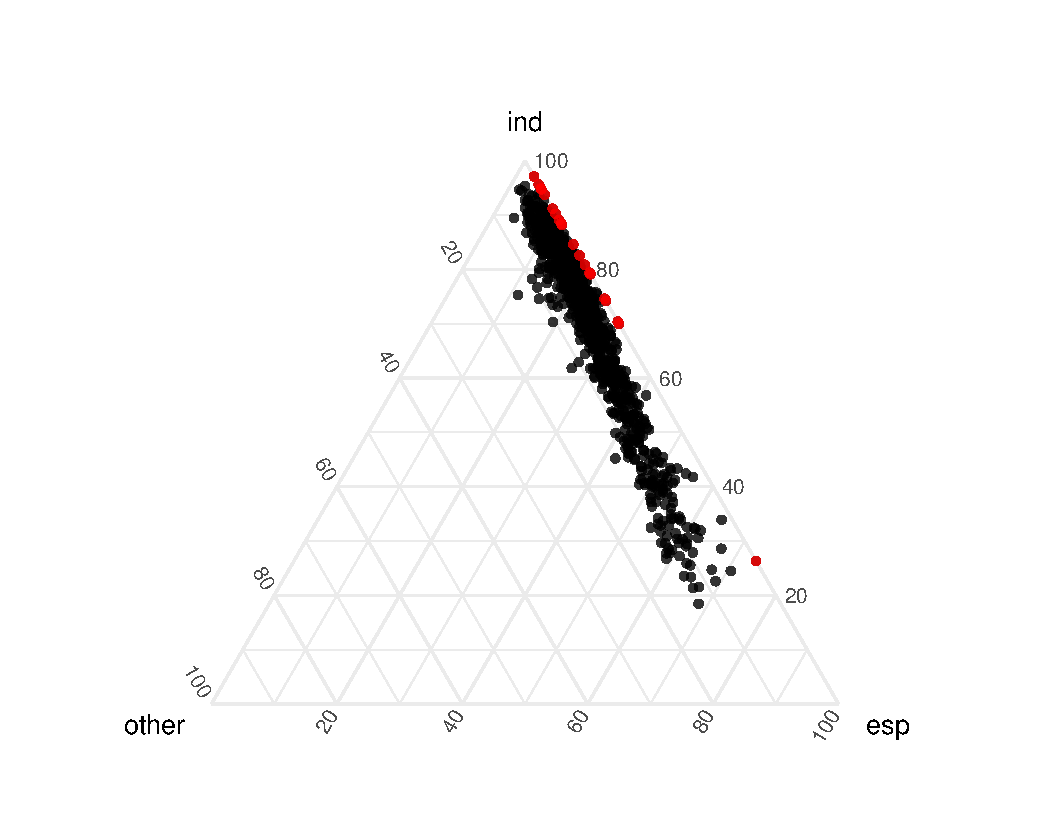
\includegraphics[trim=0cm 0cm 0cm 0cm,width=1.2\textwidth]{ternary_original.pdf}
\end{figure}
\end{column}
\begin{column}{0.5\textwidth}
\begin{itemize}
\item Most municipalities lie between \textbf{ind} and \textbf{esp} parties.
\item Some municipalities have some count zero (${\color{RED}\bullet}$).
\item<2>[$\rightarrow$] \textbf{We will deal with zeros first.}
\end{itemize}
\end{column}
\end{columns}

\end{frame}



\begin{frame}{Dealing with zeros}

Here, we consider two different approaches: \begin{itemize}\item Geometric Bayesian multiplicative (Martín-Fernández, 2015), and \item Dirichlet-multinomial smoothing after replacing by the expected posterior probabilities.\end{itemize}%

\begin{columns}
\begin{column}{0.45\textwidth}
\begin{figure}\vspace{-0.20cm}
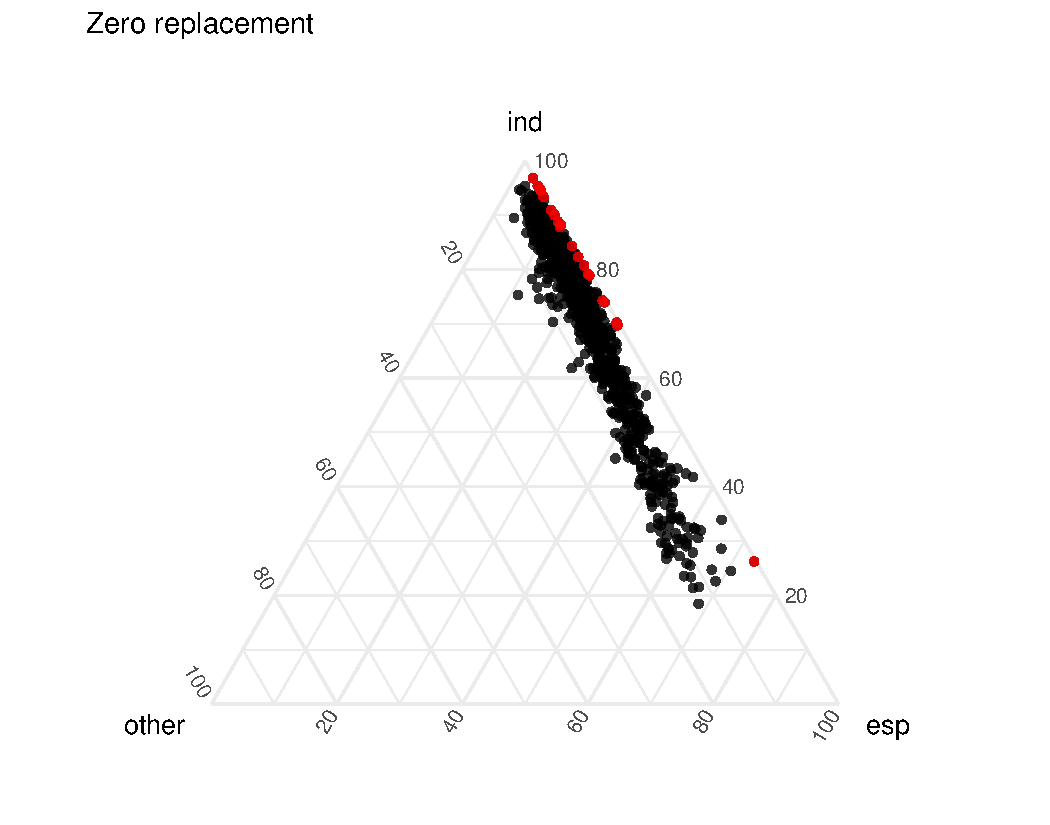
\includegraphics[trim=0cm 0cm 0cm 0cm,width=\textwidth]{ternary_zr.pdf}
\end{figure}
\end{column}
\begin{column}{0.45\textwidth}
\begin{figure}\vspace{-0.20cm}
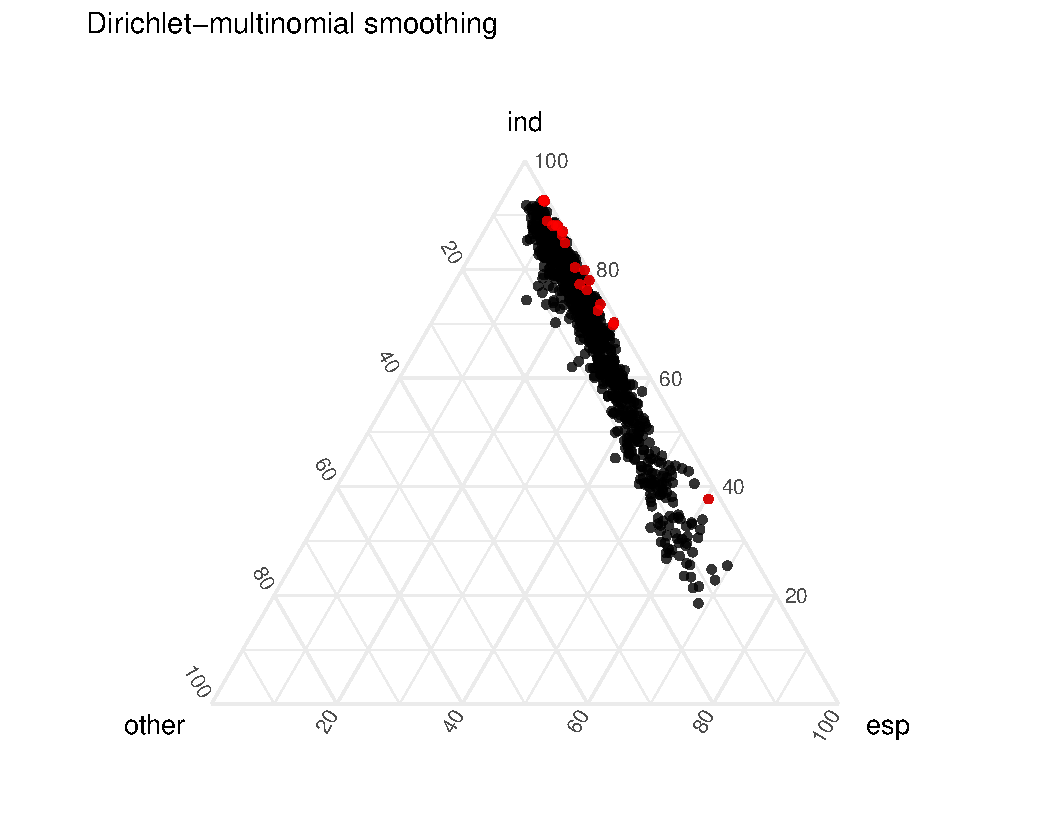
\includegraphics[trim=0cm 0cm 0cm 0cm,width=\textwidth]{ternary_nz.pdf}
\end{figure}
\end{column}
\end{columns}

\end{frame}

\begin{frame}[t]{Dealing with zeros}

\begin{columns}
\begin{column}{0.5\textwidth}
\begin{figure}\vspace{-0.20cm}
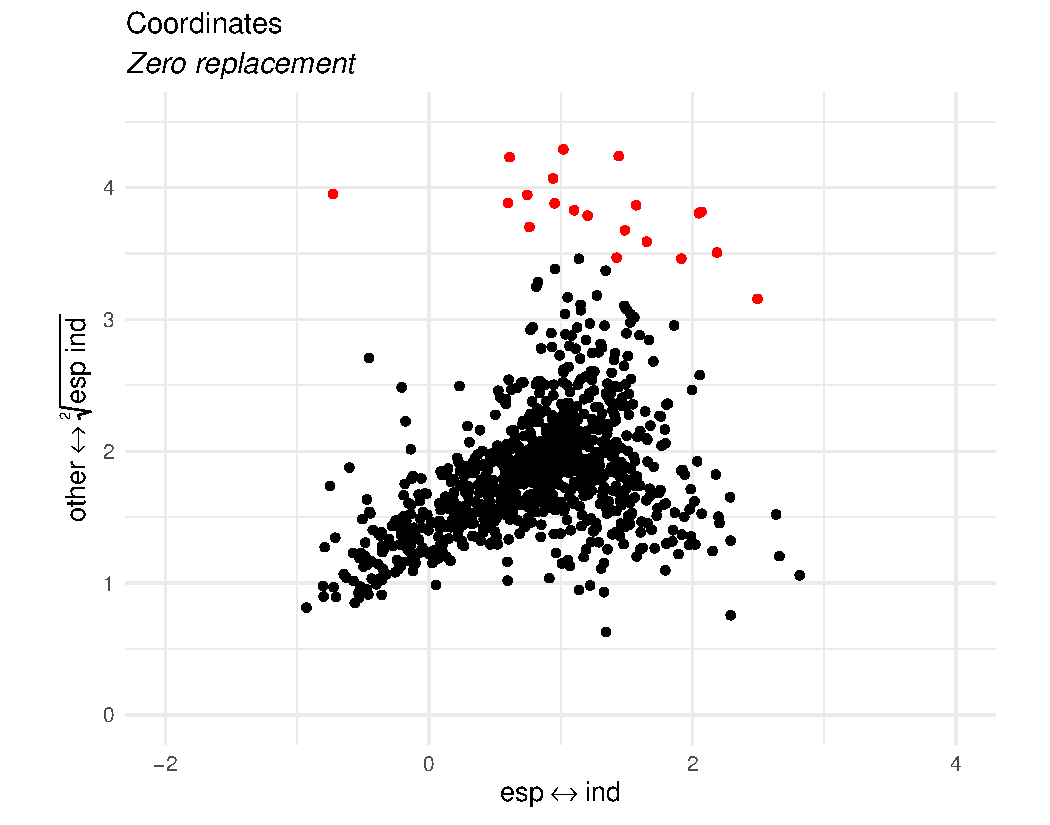
\includegraphics[trim=0cm 0cm 0cm 0cm,width=\textwidth]{coordinates_zr.pdf}
\end{figure}
\end{column}
\begin{column}{0.5\textwidth}
\begin{figure}\vspace{-0.20cm}
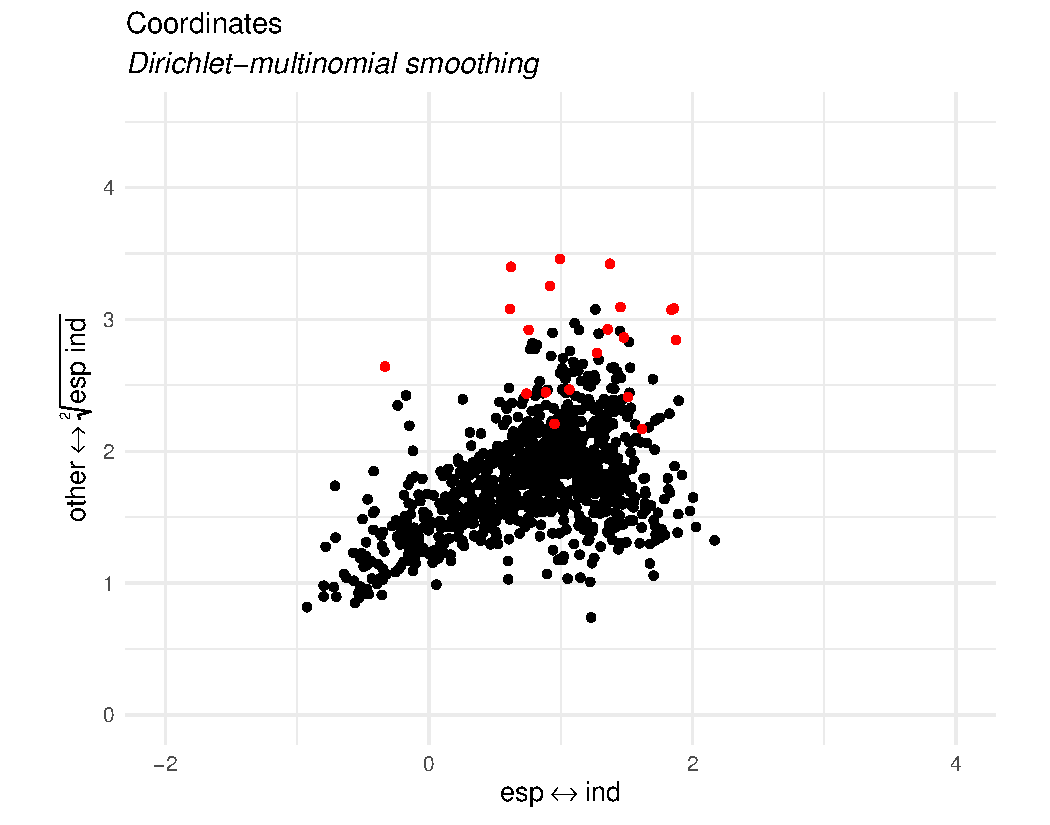
\includegraphics[trim=0cm 0cm 0cm 0cm,width=\textwidth]{coordinates_nz.pdf}
\end{figure}
\end{column}
\end{columns}

\begin{table}[H]
\centering\begingroup\fontsize{7}{9}\selectfont

\begin{tabular}{lrrr}
\toprule
Basis $\mathcal{B}$ & ind & esp & other\\
\midrule
B1 & 1 & -1 & 0\\
B2 & 1 & 1 & -1\\
\bottomrule
\end{tabular}
\endgroup{}
\end{table}


\end{frame}

\begin{frame}[t]{Clustering directly in count data}

\begin{columns}
\begin{column}{0.5\textwidth}
\begin{figure}\vspace{-0.20cm}
\only<1>{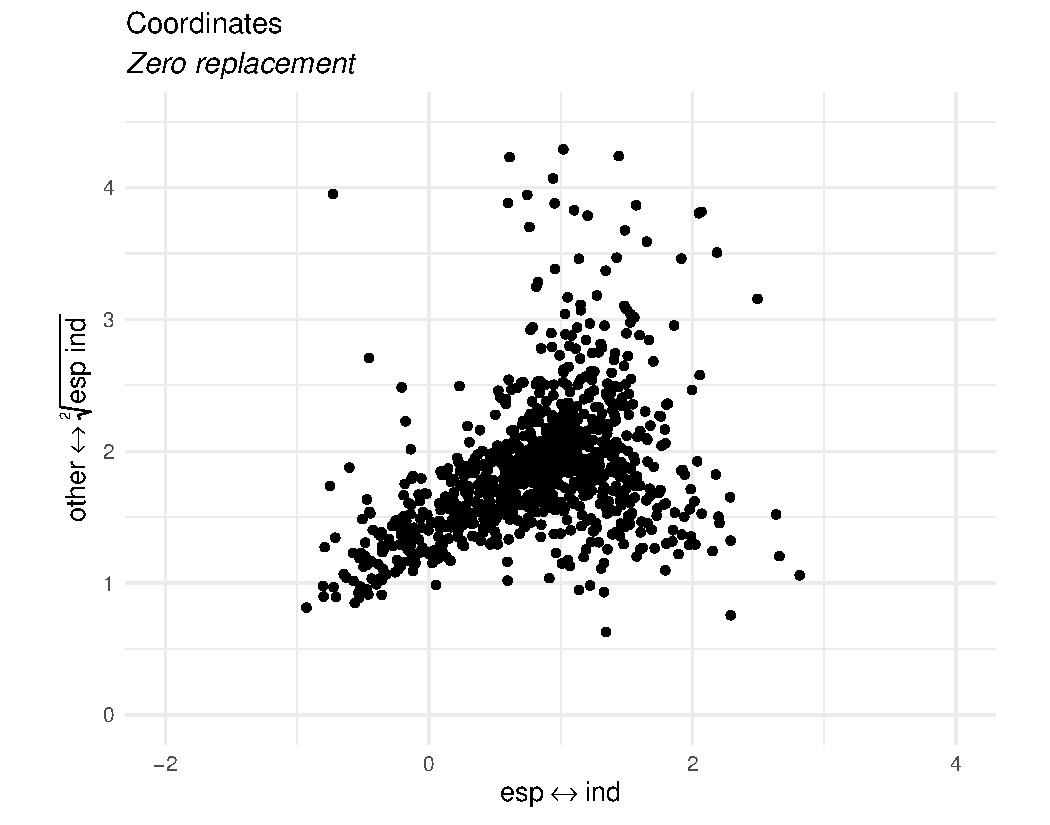
\includegraphics[trim=0cm 0cm 0cm 0cm,width=\textwidth]{coordinates_black_zr.pdf}}%
\only<2-3>{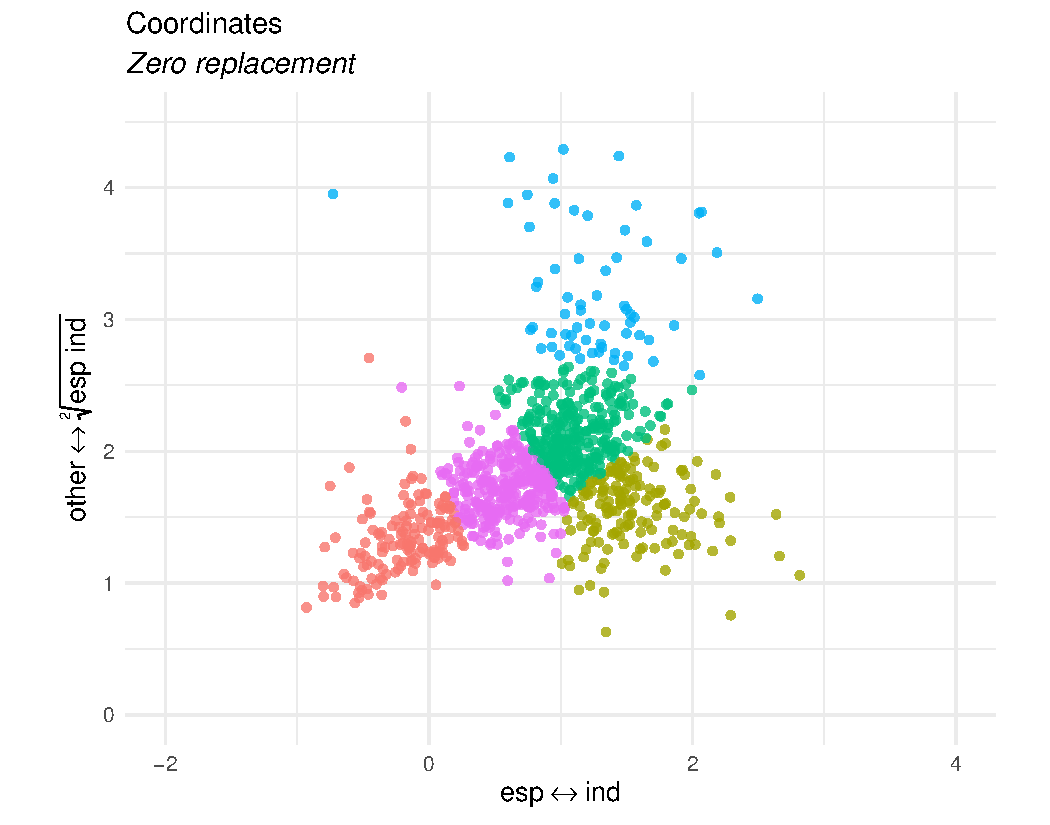
\includegraphics[trim=0cm 0cm 0cm 0cm,width=\textwidth]{clustering0_zr.pdf}}
\end{figure}
\end{column}
\begin{column}{0.5\textwidth}
\begin{figure}\vspace{-0.20cm}
\only<1>{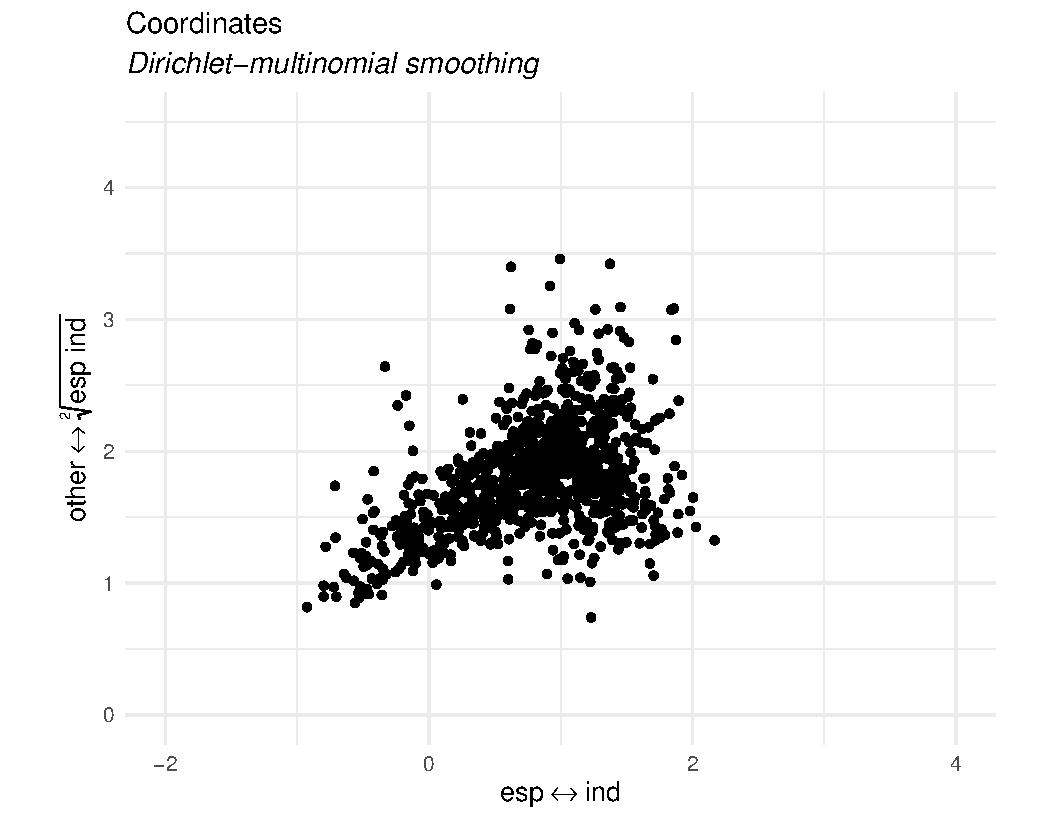
\includegraphics[trim=0cm 0cm 0cm 0cm,width=\textwidth]{coordinates_black_nz.pdf}}%
\only<2-3>{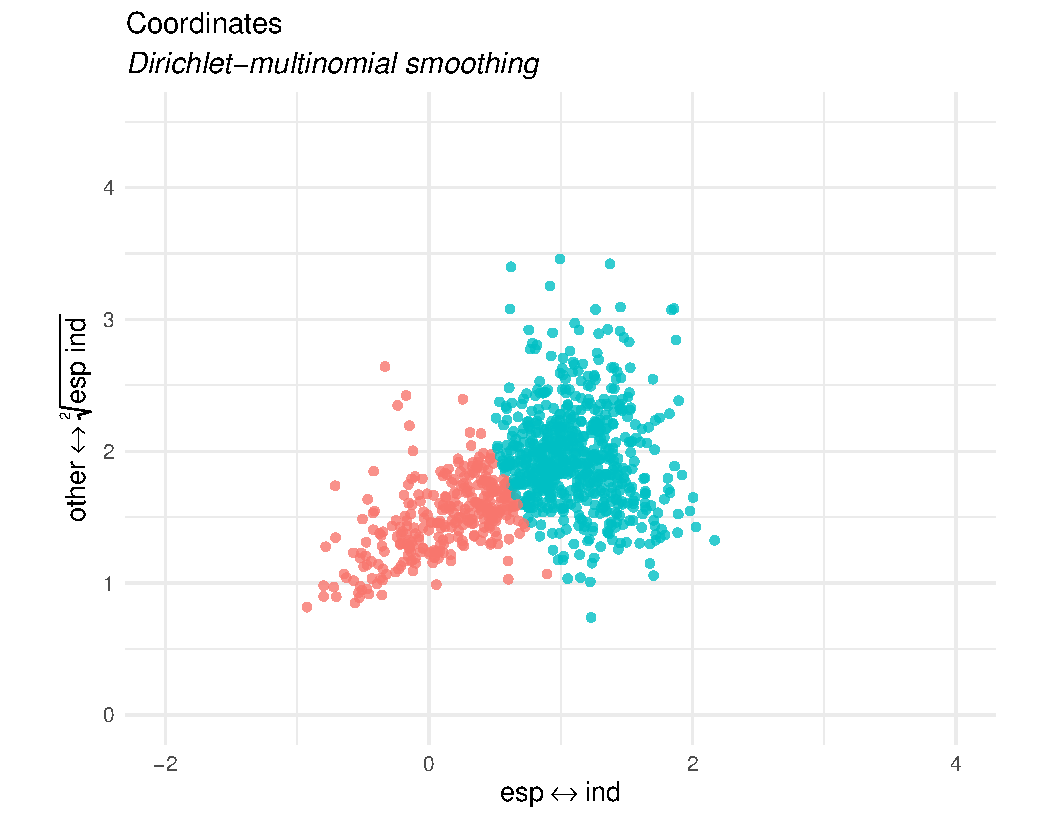
\includegraphics[trim=0cm 0cm 0cm 0cm,width=\textwidth]{clustering0_nz.pdf}}
\end{figure}
\end{column}
\end{columns}

\vspace{-0.26cm}
\only<1-2>{We can cluster our compositional data for example using $k$-means. \begin{itemize}\item  Duda-Hart test was used to discard one cluster. \item Calinski-Harabasz index was used to select $k$ between 2 and 10. \end{itemize}}
\only<3>{\begin{alertblock}{Limitations}\begin{itemize}\item In the zero-replacement approach, observations with a small amount of counts tend to create clusters.\item In DM smoothing results can be affected by the Dirichlet prior.\end{itemize}\end{alertblock}}
\end{frame}

\begin{frame}[t]{Compositional variability}

\begin{columns}
\begin{column}{0.5\textwidth}
\begin{figure}\vspace{-0.20cm}%
\only<1>{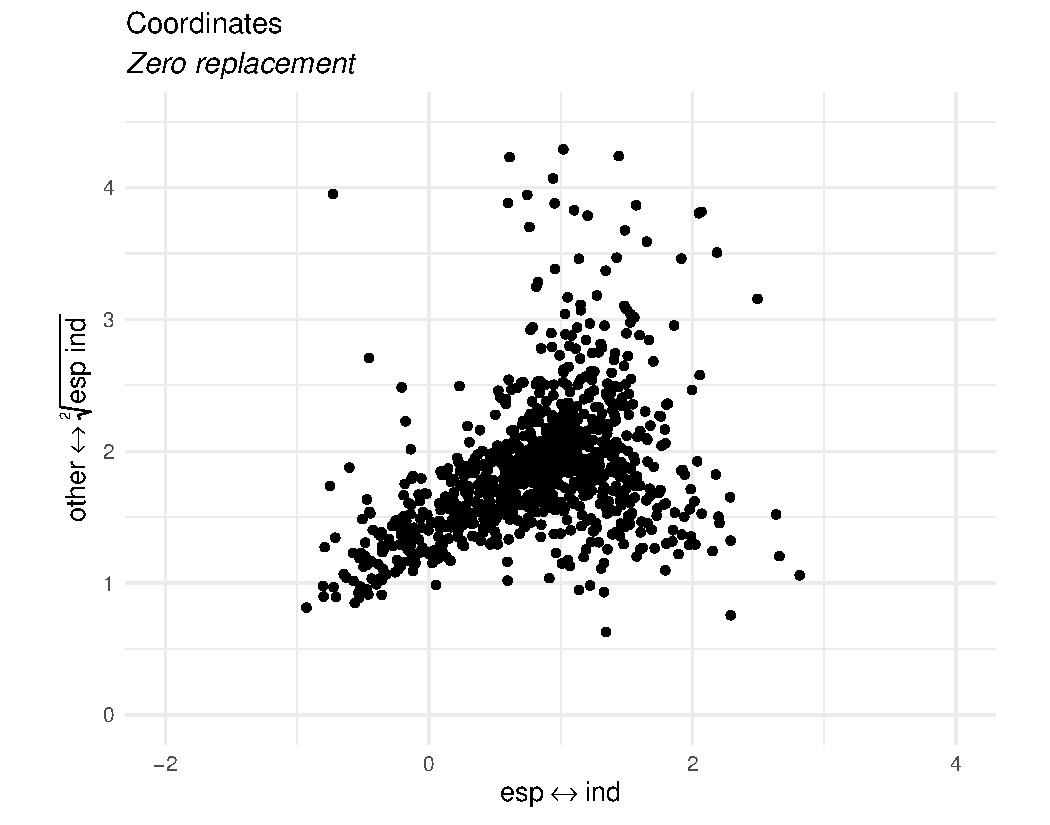
\includegraphics[trim=0cm 0cm 0cm 0cm,width=\textwidth]{coordinates_black_zr.pdf}}%
\only<2>{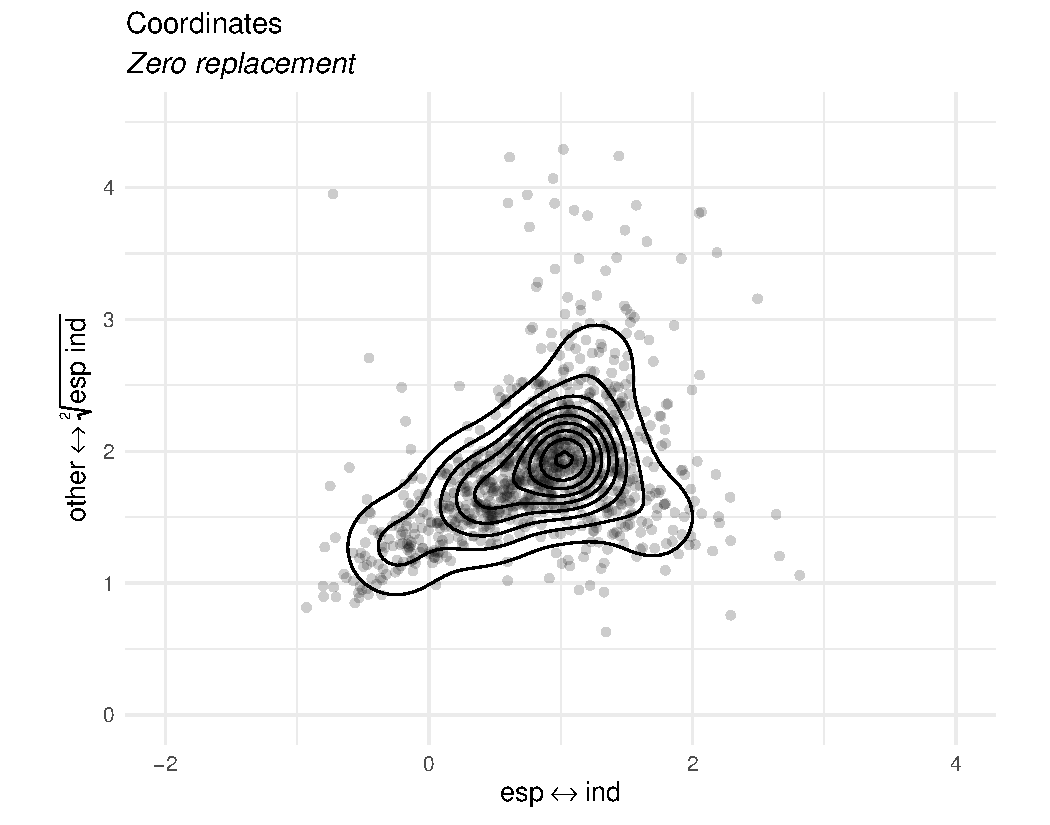
\includegraphics[trim=0cm 0cm 0cm 0cm,width=\textwidth]{model_zr.pdf}}%
\end{figure}
\end{column}
\begin{column}{0.5\textwidth}%
\begin{figure}\vspace{-0.20cm}
\only<1>{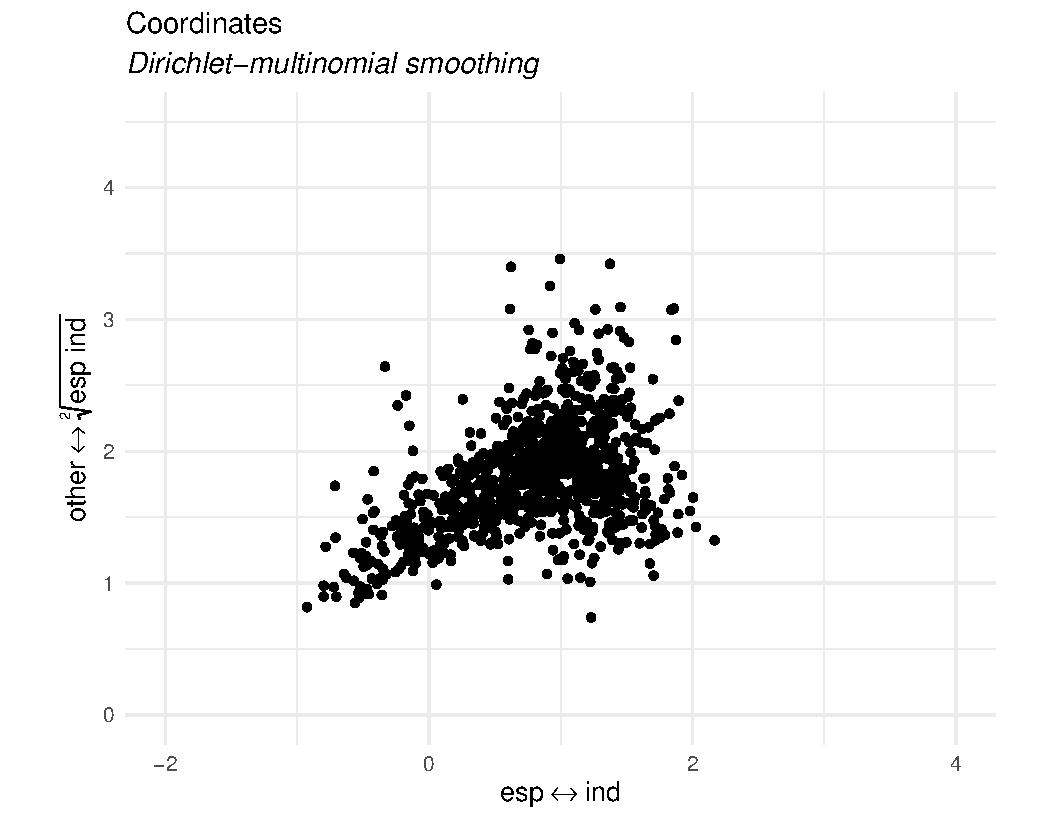
\includegraphics[trim=0cm 0cm 0cm 0cm,width=\textwidth]{coordinates_black_nz.pdf}}%
\only<2>{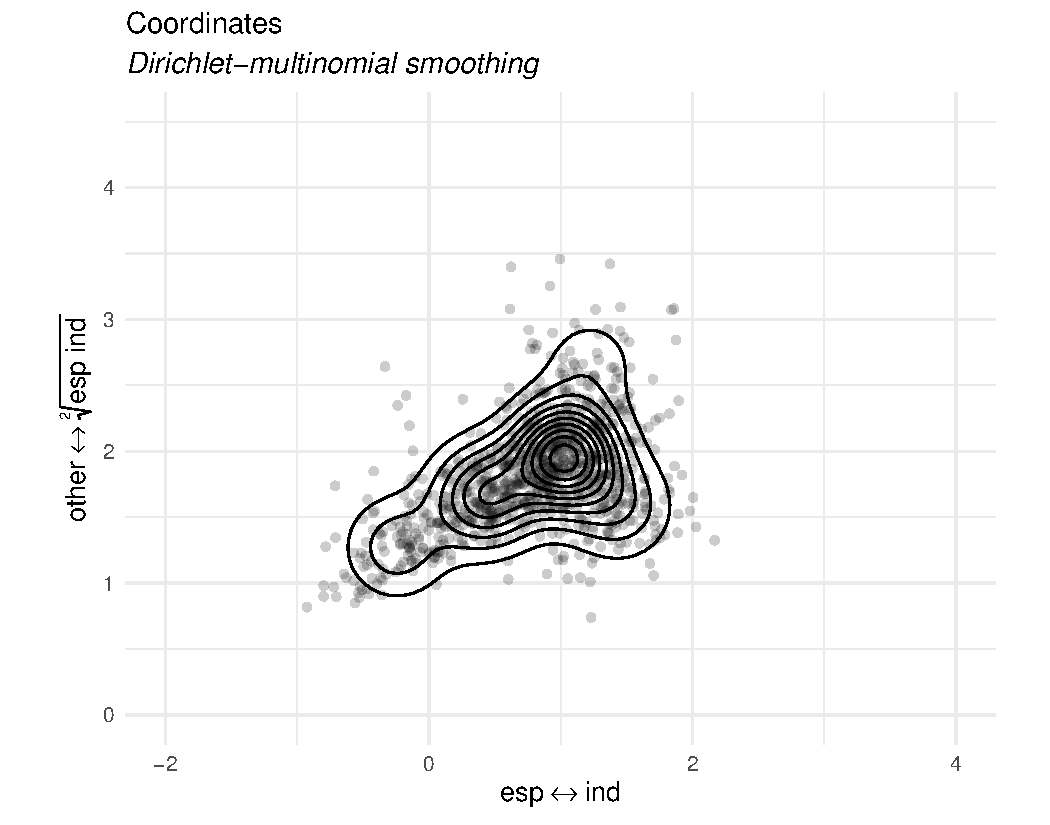
\includegraphics[trim=0cm 0cm 0cm 0cm,width=\textwidth]{model_nz.pdf}}%
\end{figure}
\end{column}
\end{columns}

\vspace{-0.26cm}
\only<1-2>{\begin{exampleblock}{Modelling using Gaussian mixtures}\vspace{0.1cm}Find a distribution to model the original sample. Mixtures of Gaussian distribution are a good option (Nguyen \& McLachlan, 2018).\begin{itemize}\item[$\rightarrow$] According to BIC criterion, a mixture of 7 and 5 spherical Gaussian distributions with equal volume were respectively used.\end{itemize}\end{exampleblock}}

\end{frame}



\begin{frame}[t]{Count variability}

\begin{columns}
\begin{column}{0.5\textwidth}
\begin{figure}\vspace{-0.20cm}
\only<1>{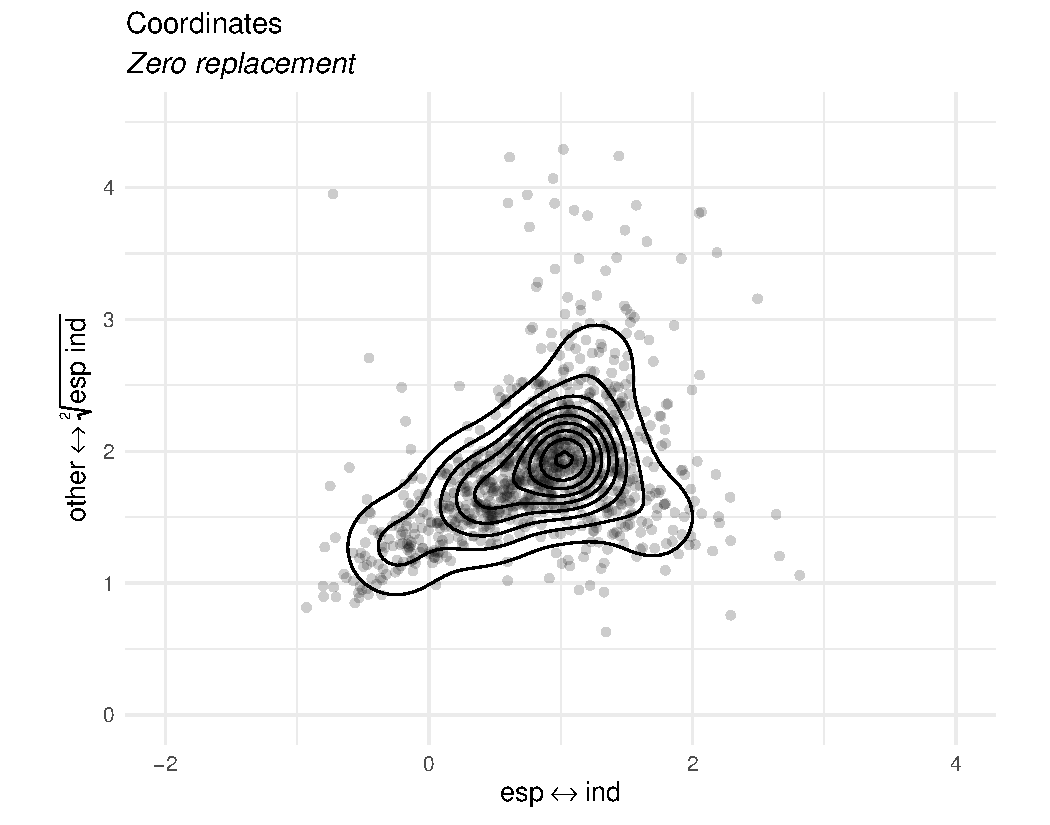
\includegraphics[trim=0cm 0cm 0cm 0cm,width=\textwidth]{model_zr.pdf}}%
\only<2>{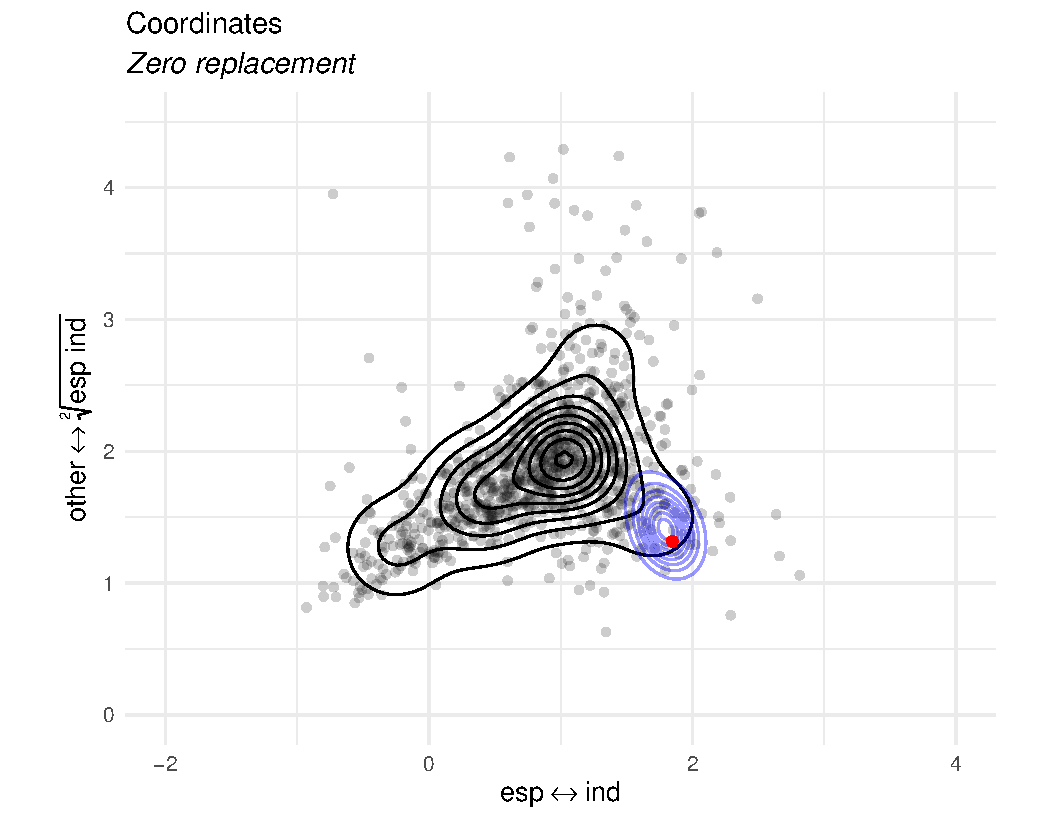
\includegraphics[trim=0cm 0cm 0cm 0cm,width=\textwidth]{posterior_zr_60.pdf}}%
\only<3>{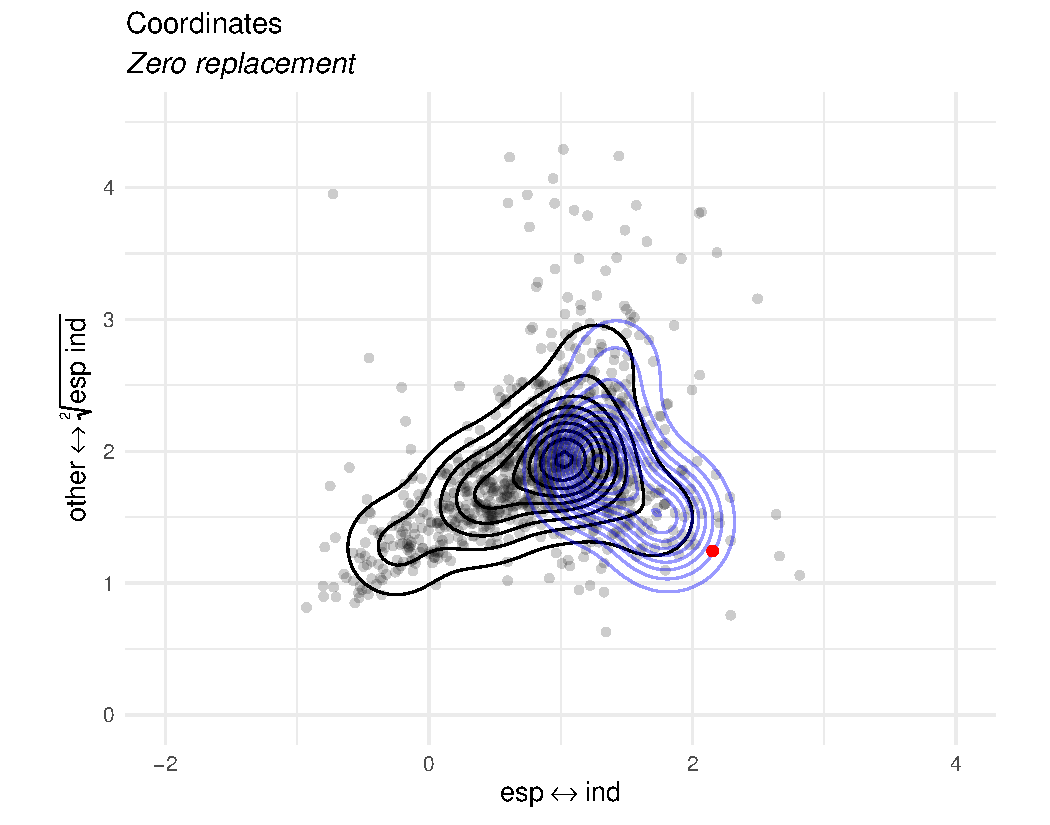
\includegraphics[trim=0cm 0cm 0cm 0cm,width=\textwidth]{posterior_zr_331.pdf}}%
\only<4>{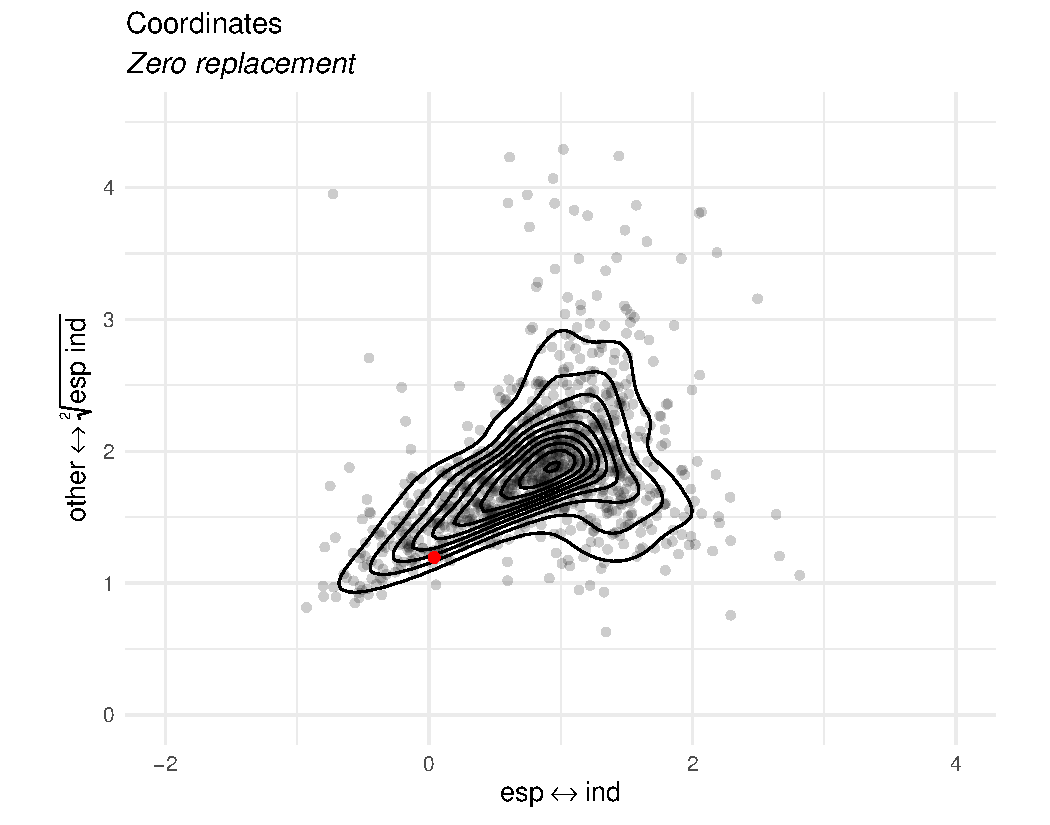
\includegraphics[trim=0cm 0cm 0cm 0cm,width=\textwidth]{posterior_zr_90.pdf}}%
\end{figure}
\end{column}
\begin{column}{0.5\textwidth}
\begin{figure}\vspace{-0.20cm}
\only<1>{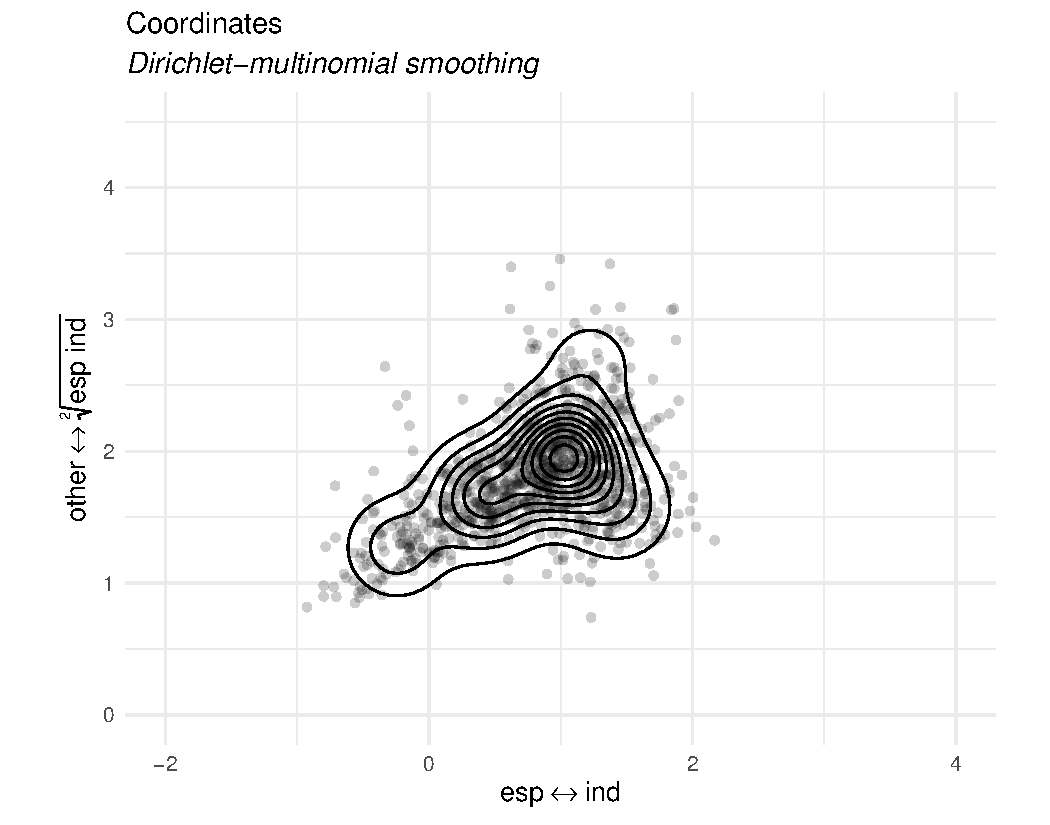
\includegraphics[trim=0cm 0cm 0cm 0cm,width=\textwidth]{model_nz.pdf}}%
\only<2>{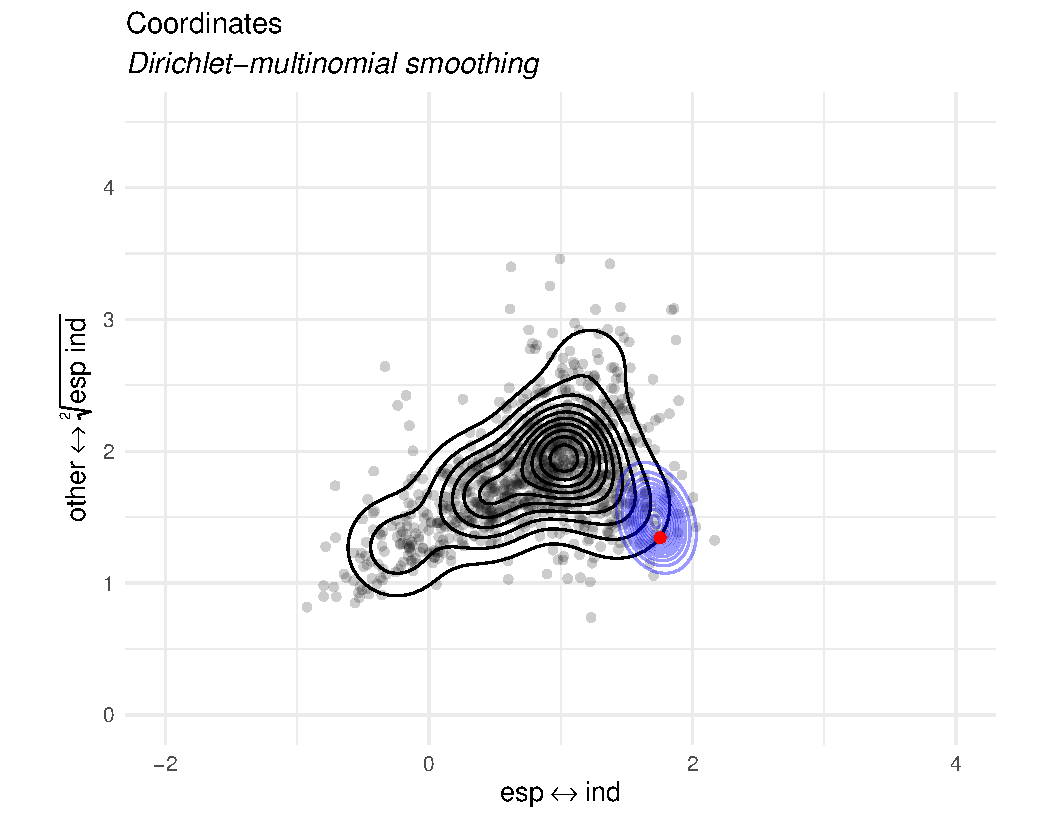
\includegraphics[trim=0cm 0cm 0cm 0cm,width=\textwidth]{posterior_nz_60.pdf}}%
\only<3>{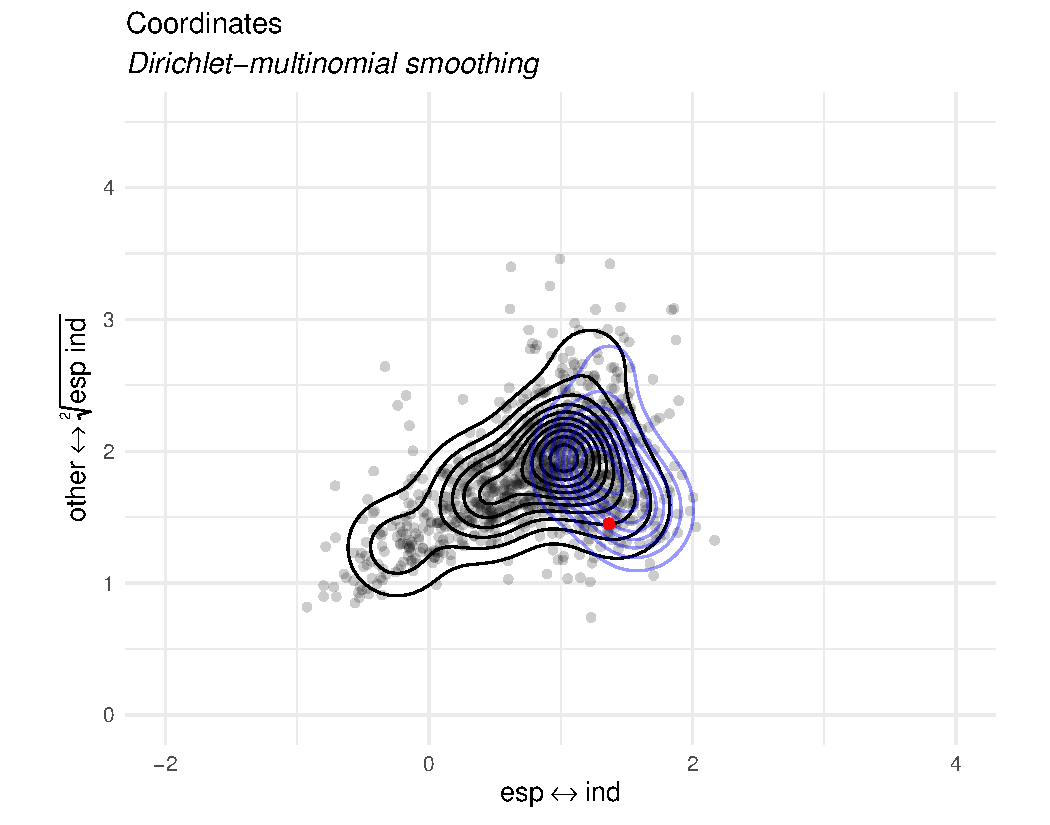
\includegraphics[trim=0cm 0cm 0cm 0cm,width=\textwidth]{posterior_nz_331.pdf}}%
\only<4>{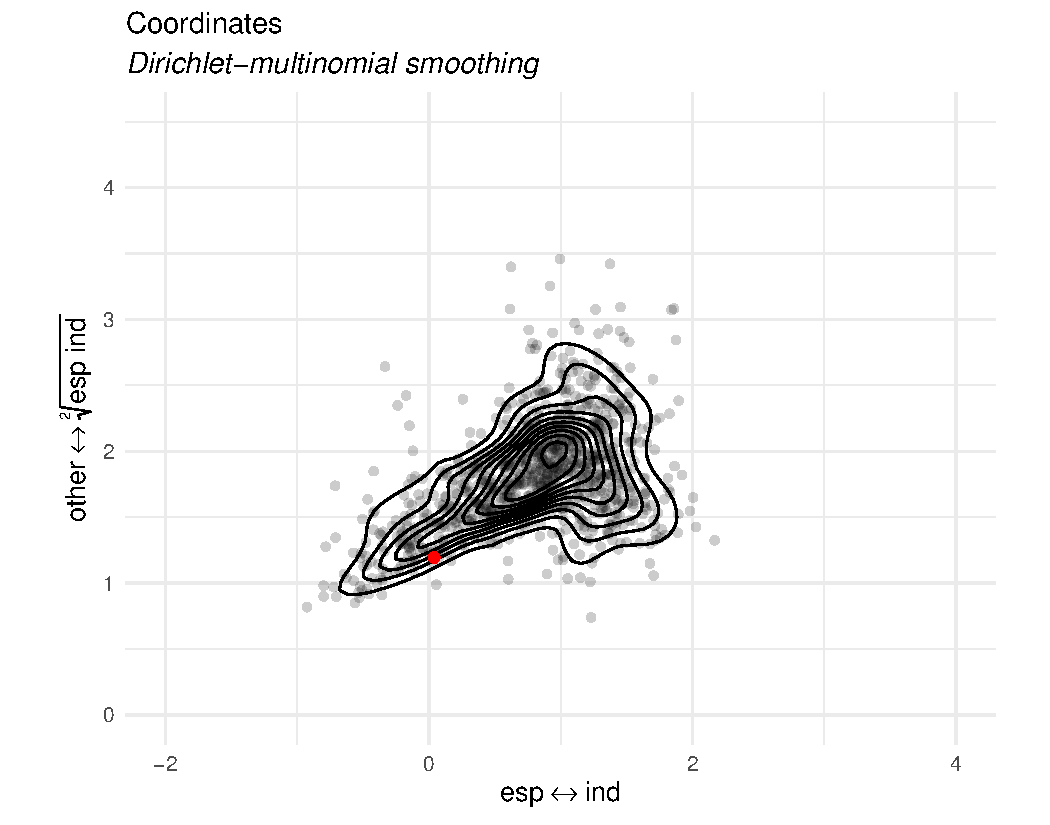
\includegraphics[trim=0cm 0cm 0cm 0cm,width=\textwidth]{posterior_nz_90.pdf}}%
\end{figure}
\end{column}
\end{columns}

\vspace{-0.2cm}
\begin{exampleblock}{Sampling from the posterior distribution}
For each count observation $\textbf{x}_i$, we sample from the posterior distribution $P(\textbf{h} \mid \textbf{x}_i; f)$, where $f$ is the mixture of Gaussian distributions.
\begin{itemize}
\item Metropolis–Hastings using $g(\textbf{h}) = f(\textbf{h})\cdot\text{Mult}(\textbf{x}_i; \textbf{ilr}_\mathcal{B}^{-1}(\textbf{h}))$ with proposal step defined by the Laplace approximation of $P(\textbf{h} \mid \textbf{x}_i; f)$ centred at zero.
\uncover<2->{
\only<1-2>{\item{$i=\text{``Argelaguer''},\; \textbf{x}_i=(\text{ind: } 259, \text{esp: } 19, \text{other: } 14)$}}%
\only<3>{\item{$i=\text{``Gisclareny''},\; \textbf{x}_i=(\text{ind: } 1, \text{esp: } 21, \text{other: } 1)$}}%
\only<4>{\item{$i=\text{``Barcelona''},\; \textbf{x}_i=(\text{ind: } 429\,782, \text{esp: } 405\,924, \text{other: } 96\,748)$}}%
}
\end{itemize}
\end{exampleblock}


\end{frame}


\begin{frame}[t]{Compositional and count variability}

\begin{columns}
\begin{column}{0.5\textwidth}
\begin{figure}\vspace{-0.20cm}%
\only<1>{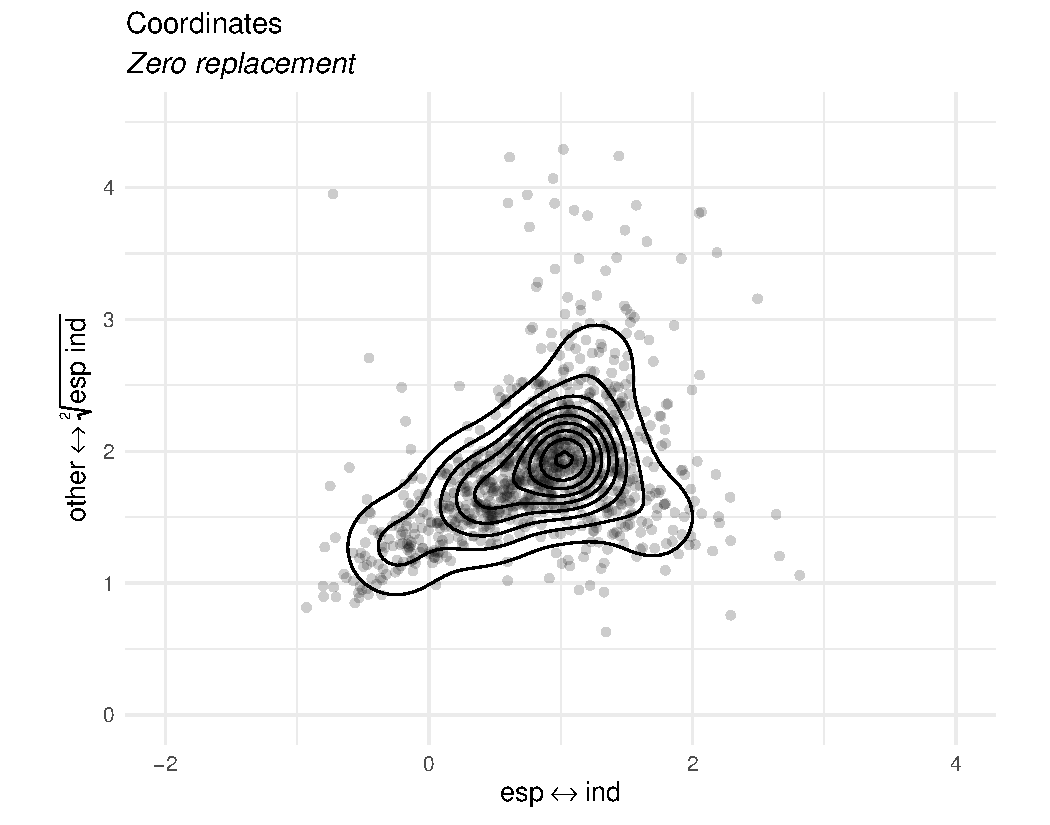
\includegraphics[trim=0cm 0cm 0cm 0cm,width=\textwidth]{model_zr.pdf}}%
\only<2>{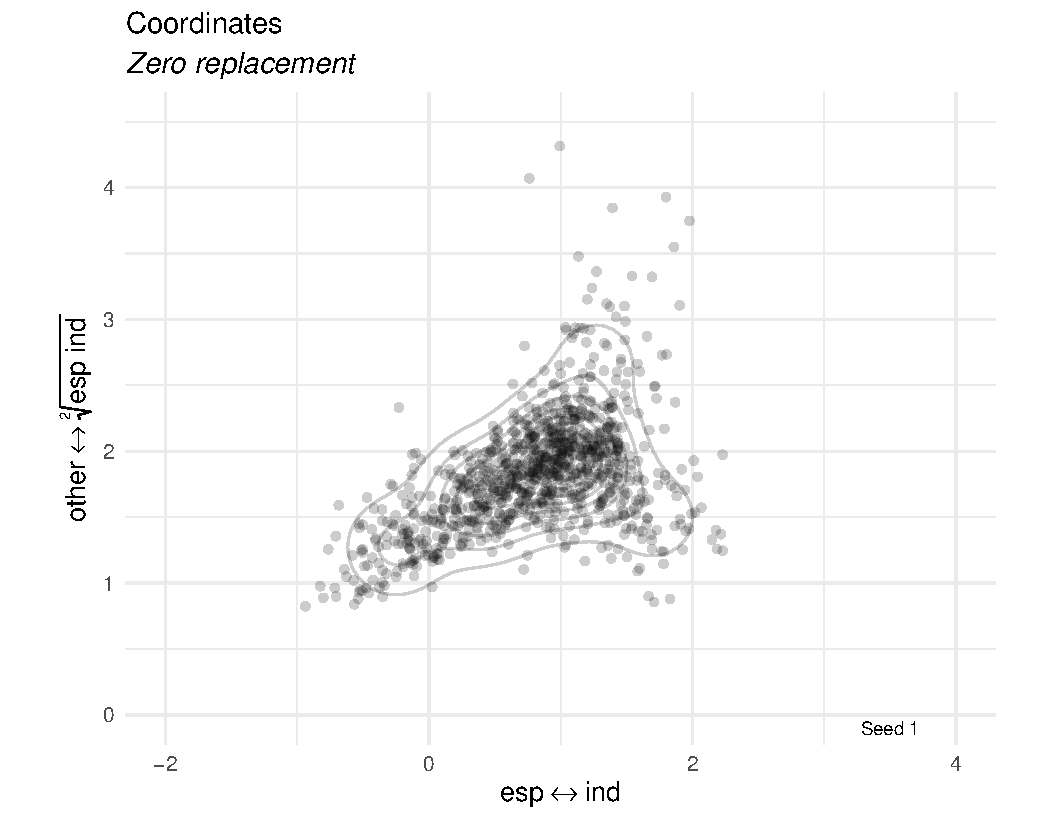
\includegraphics[trim=0cm 0cm 0cm 0cm,width=\textwidth]{sample_zr_1.pdf}}%
\only<3>{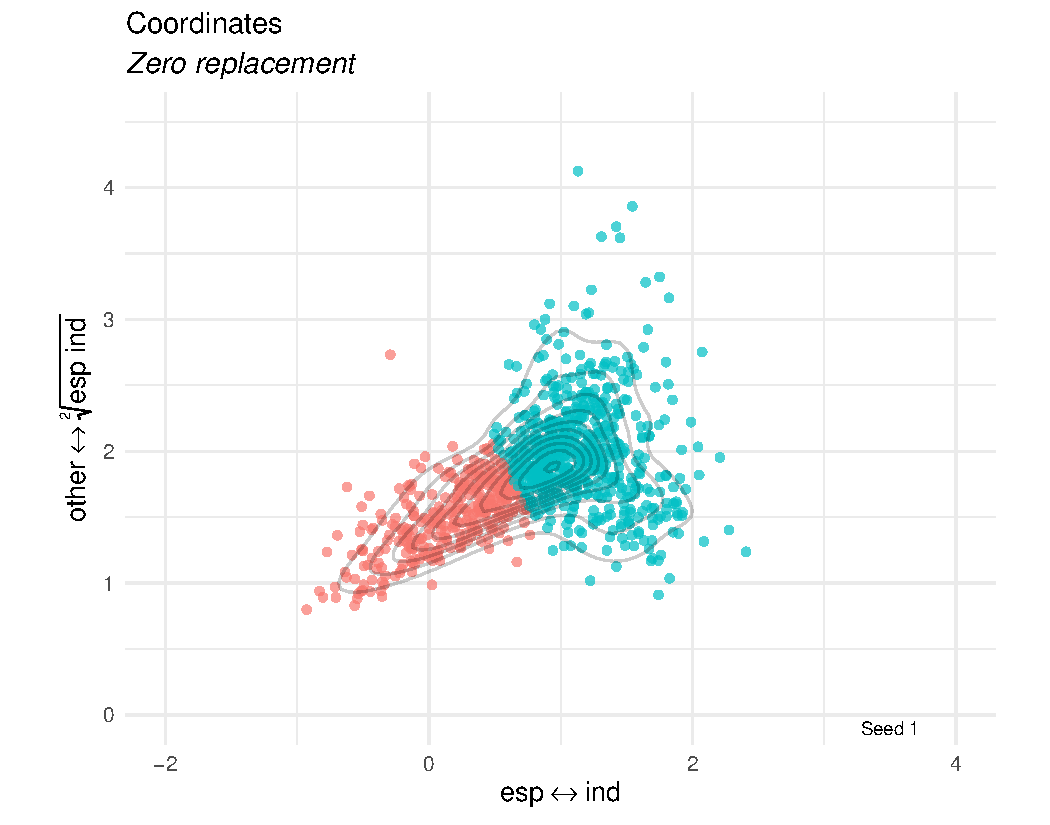
\includegraphics[trim=0cm 0cm 0cm 0cm,width=\textwidth]{sample_cl_zr_1.pdf}}%
\only<4>{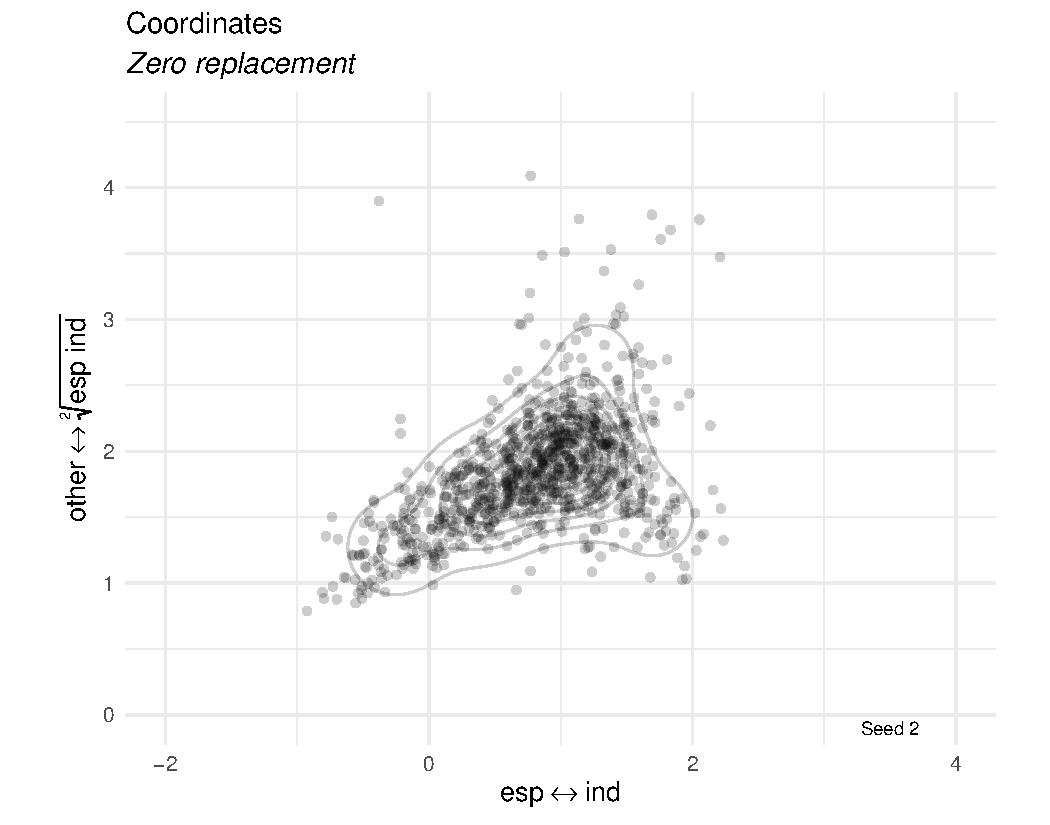
\includegraphics[trim=0cm 0cm 0cm 0cm,width=\textwidth]{sample_zr_2.pdf}}%
\only<5>{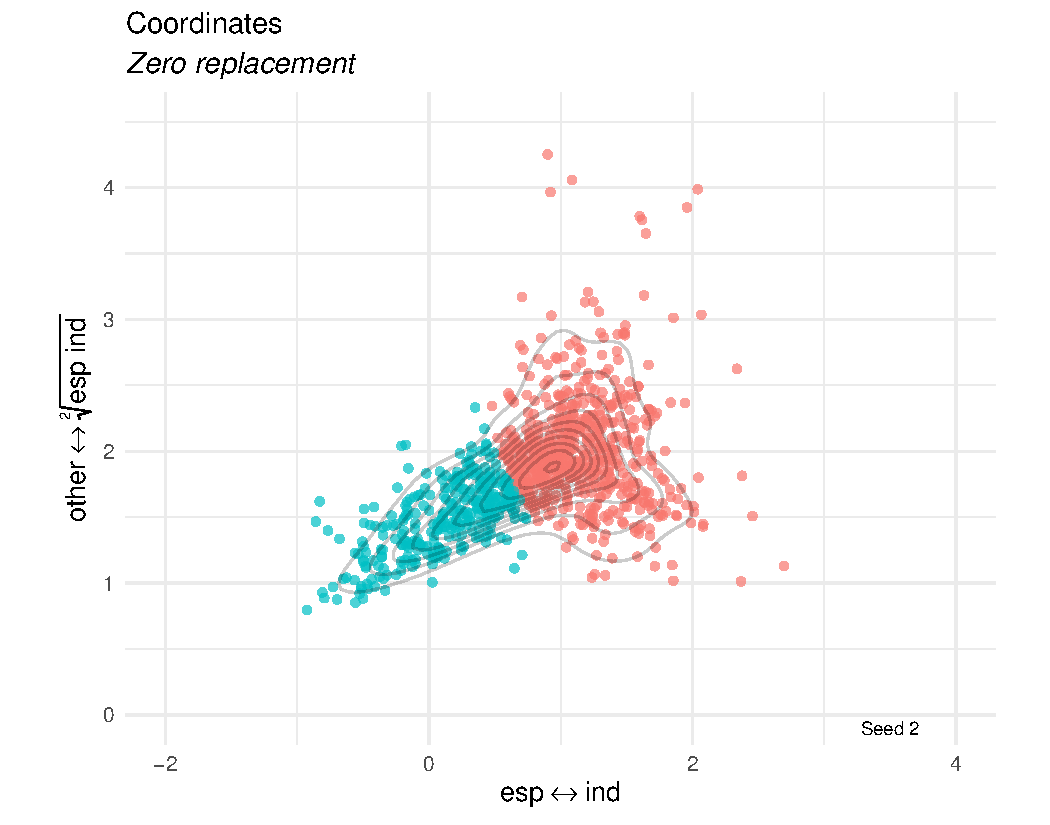
\includegraphics[trim=0cm 0cm 0cm 0cm,width=\textwidth]{sample_cl_zr_2.pdf}}%
\only<6>{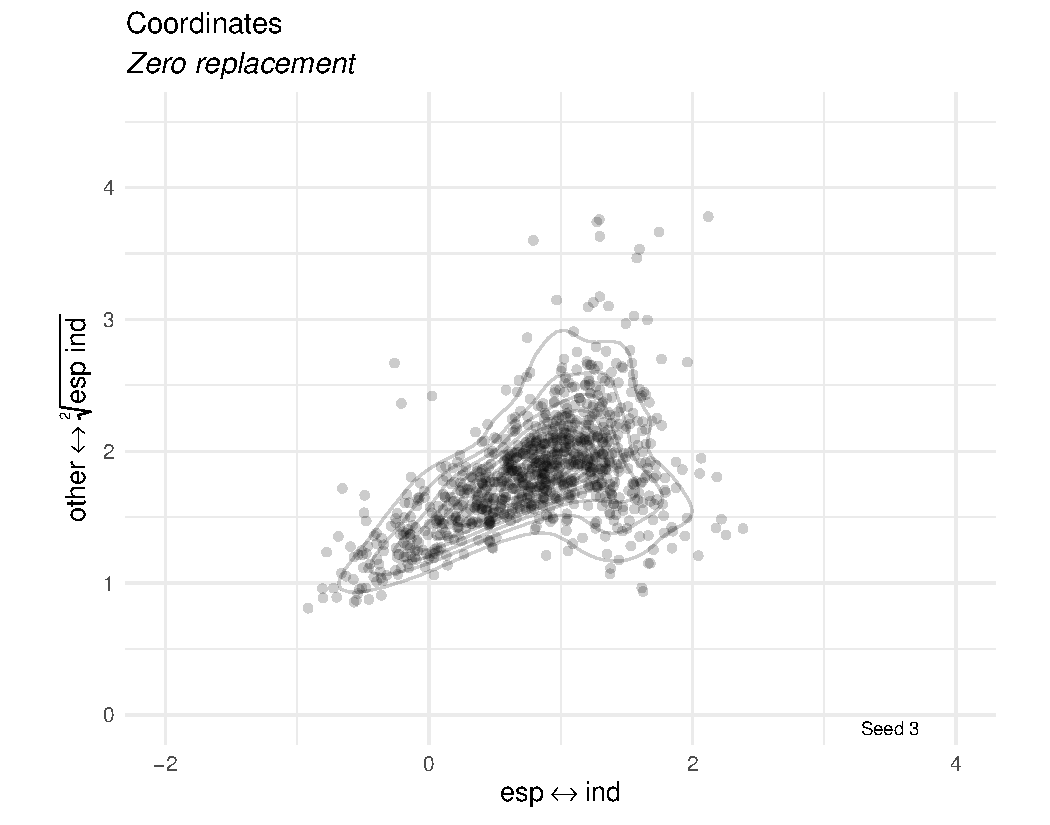
\includegraphics[trim=0cm 0cm 0cm 0cm,width=\textwidth]{sample_zr_3.pdf}}%
\only<7>{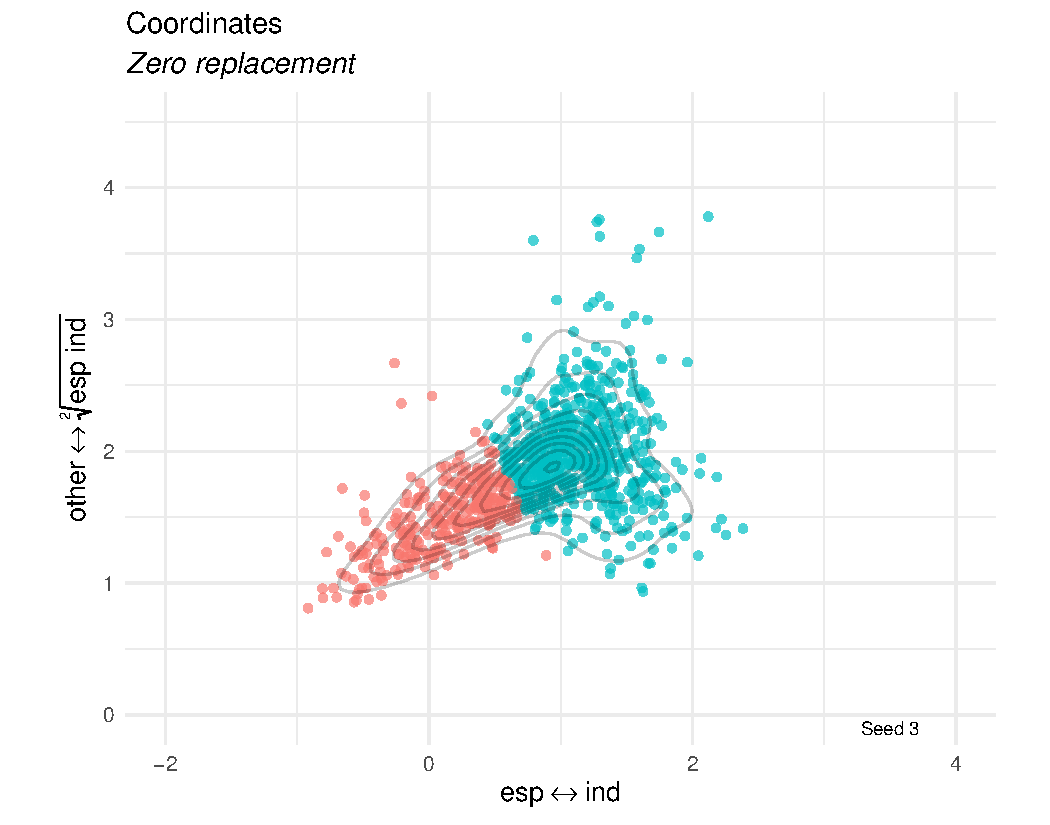
\includegraphics[trim=0cm 0cm 0cm 0cm,width=\textwidth]{sample_cl_zr_3.pdf}}%
\only<8>{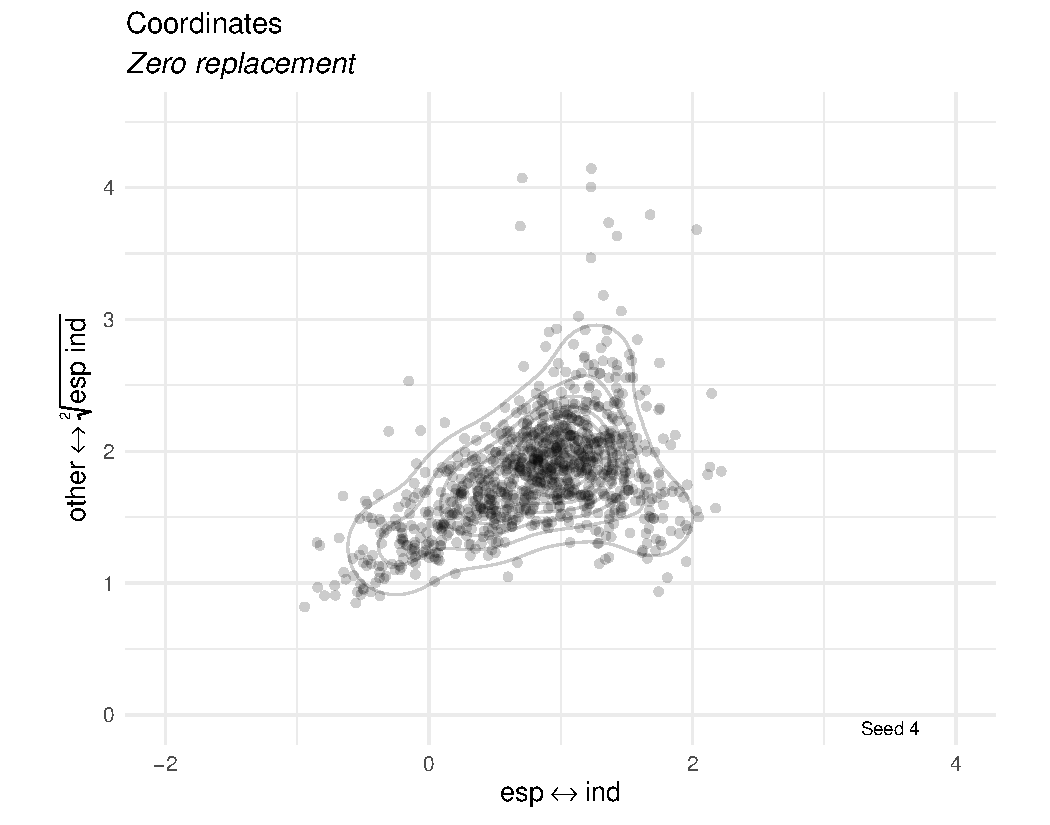
\includegraphics[trim=0cm 0cm 0cm 0cm,width=\textwidth]{sample_zr_4.pdf}}%
\only<9>{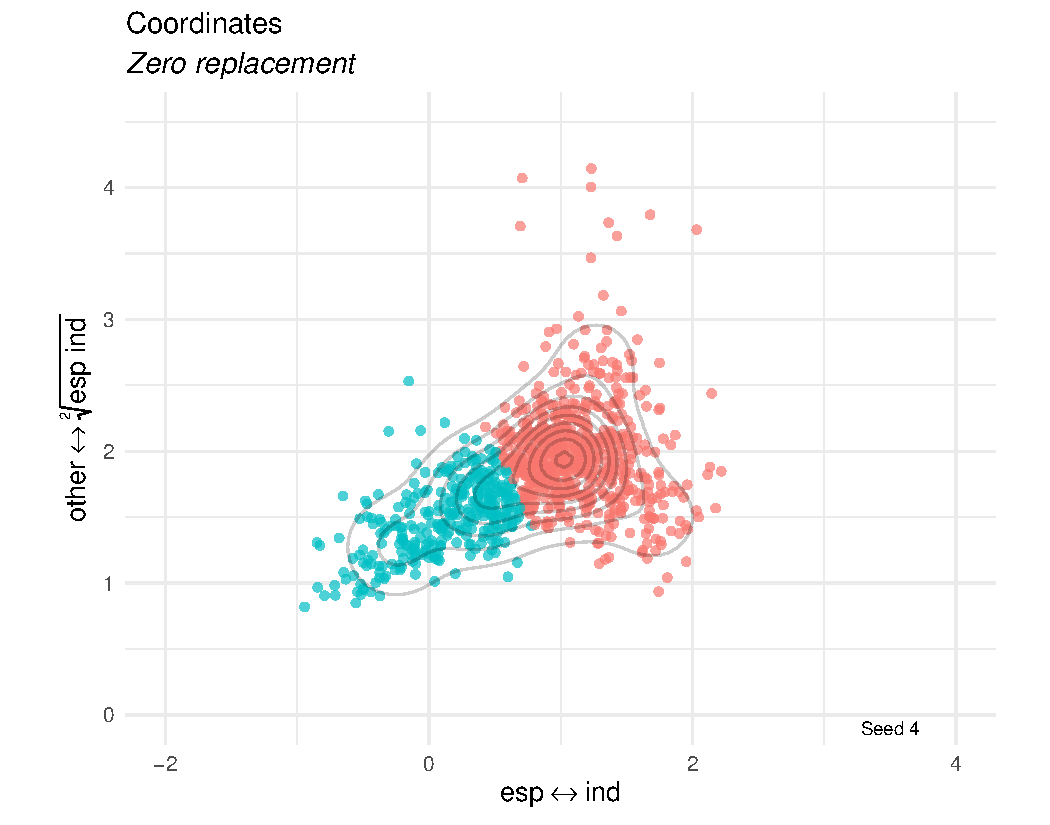
\includegraphics[trim=0cm 0cm 0cm 0cm,width=\textwidth]{sample_cl_zr_4.pdf}}%
\end{figure}
\end{column}
\begin{column}{0.5\textwidth}%
\begin{figure}\vspace{-0.20cm}
\only<1>{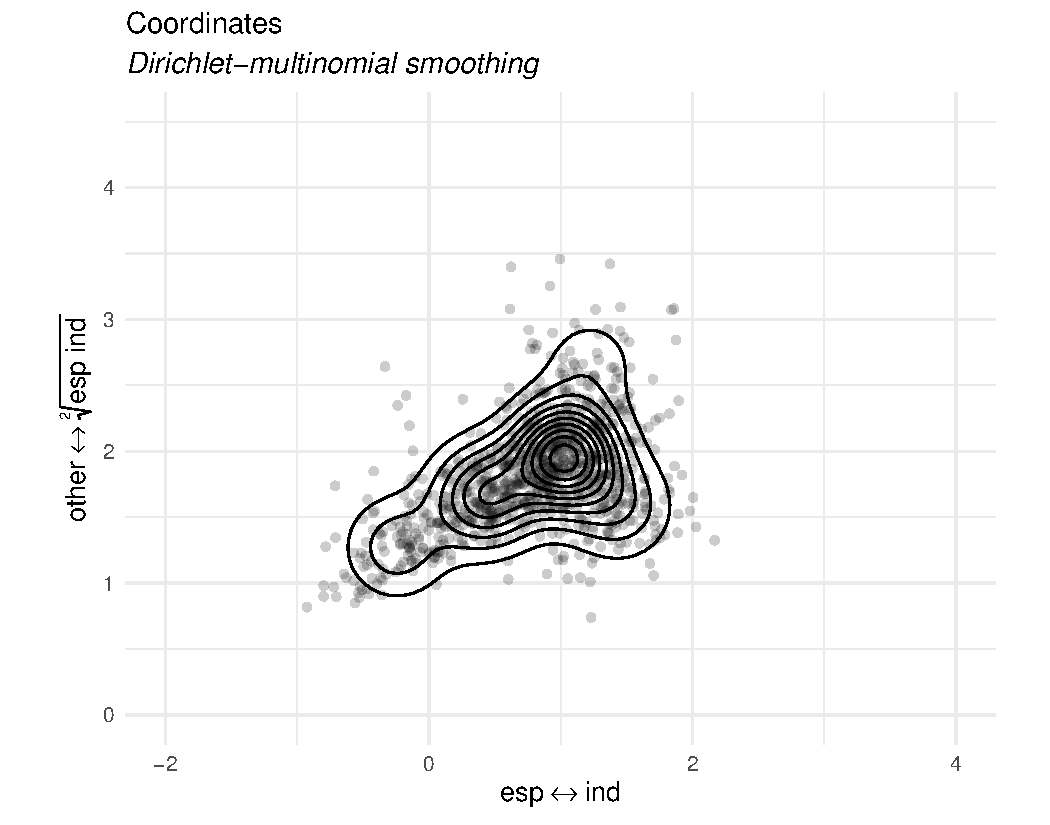
\includegraphics[trim=0cm 0cm 0cm 0cm,width=\textwidth]{model_nz.pdf}}%
\only<2>{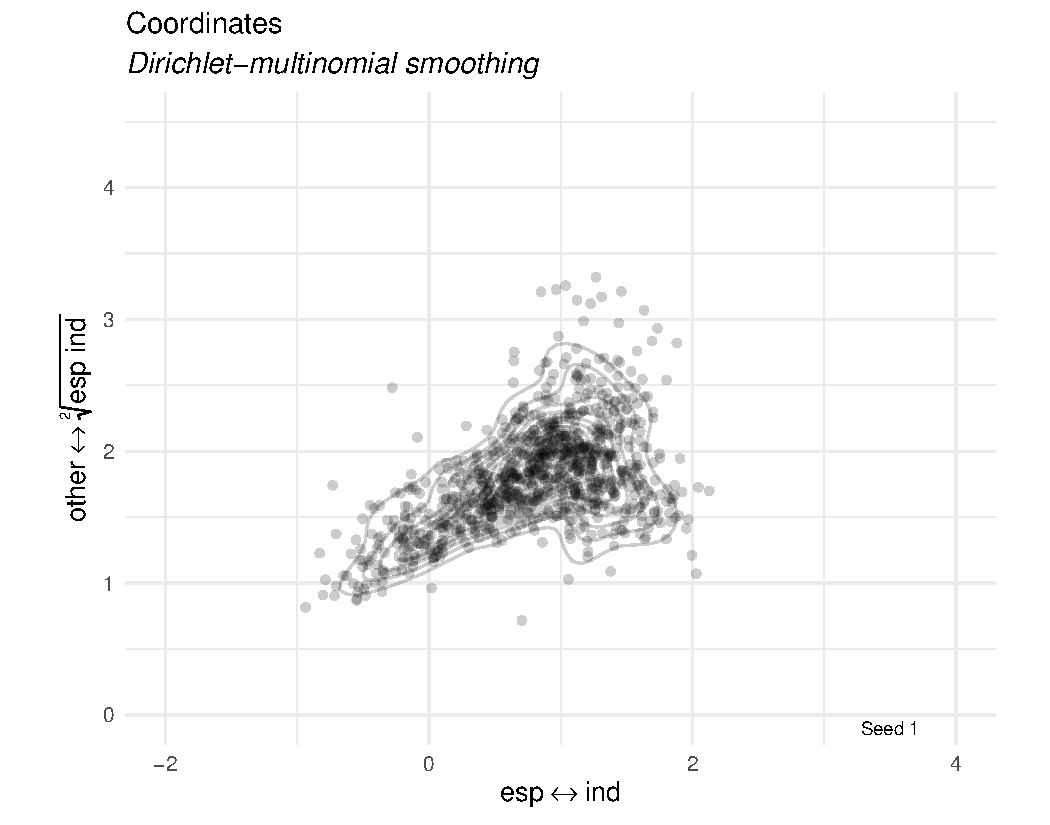
\includegraphics[trim=0cm 0cm 0cm 0cm,width=\textwidth]{sample_nz_1.pdf}}%
\only<3>{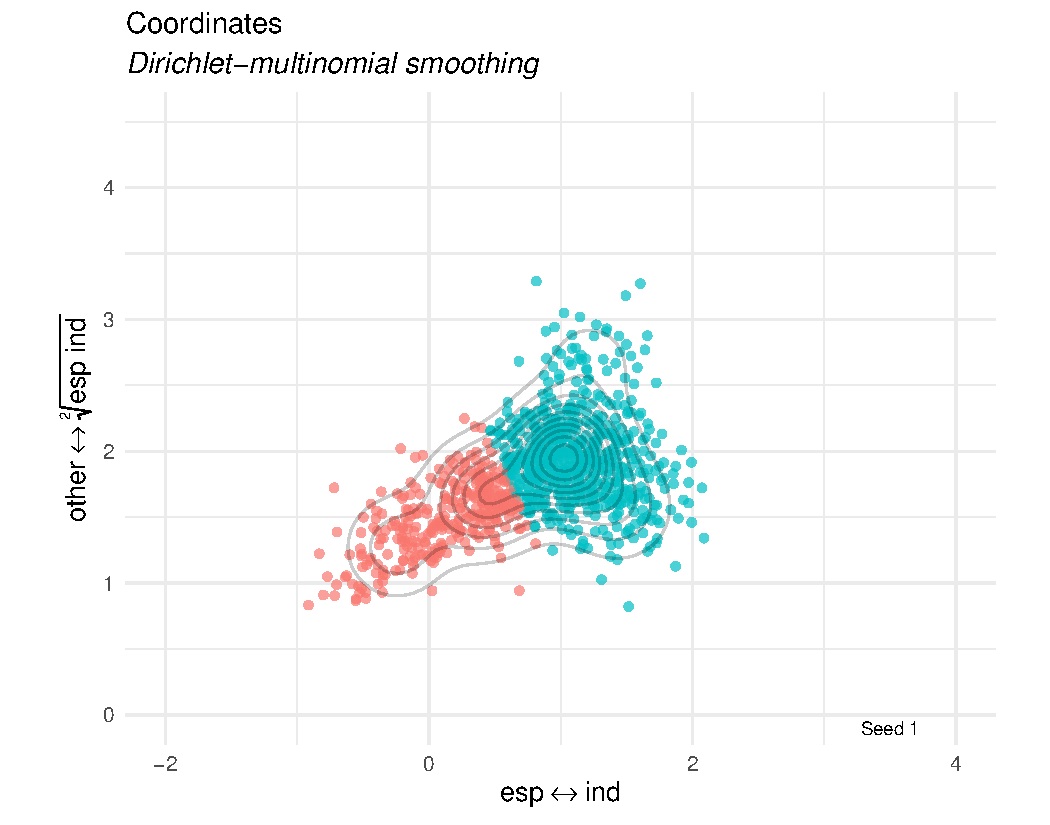
\includegraphics[trim=0cm 0cm 0cm 0cm,width=\textwidth]{sample_cl_nz_1.pdf}}%
\only<4>{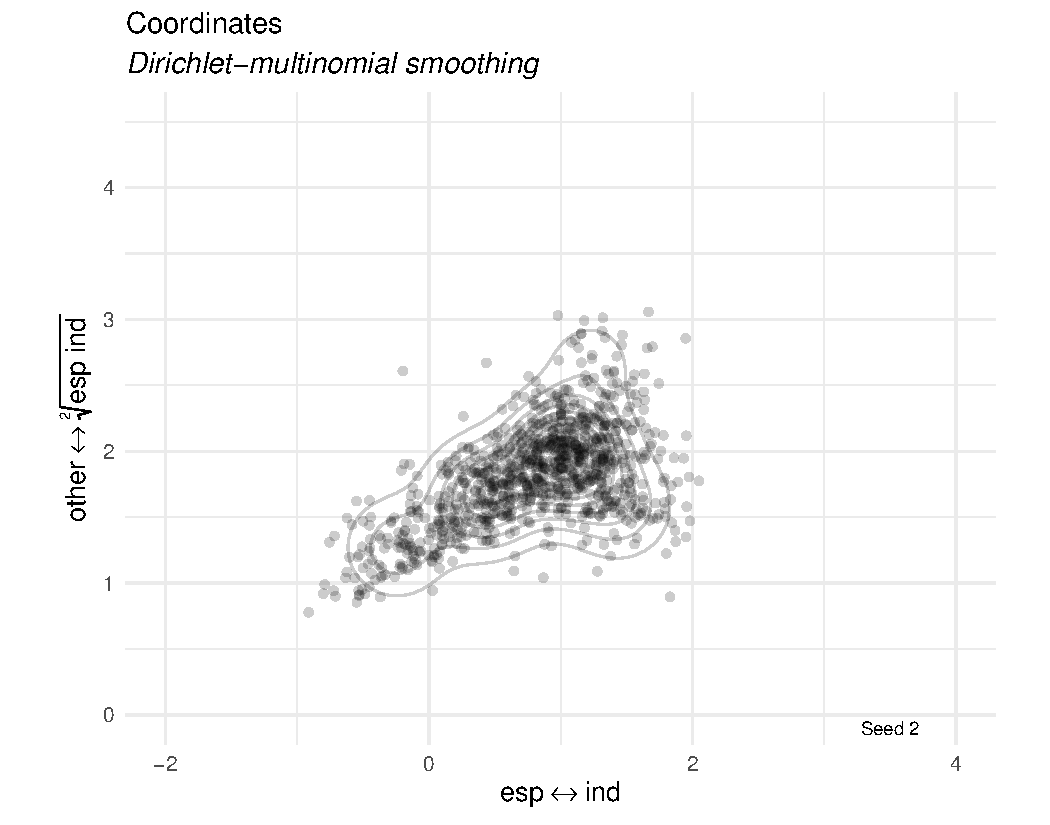
\includegraphics[trim=0cm 0cm 0cm 0cm,width=\textwidth]{sample_nz_2.pdf}}%
\only<5>{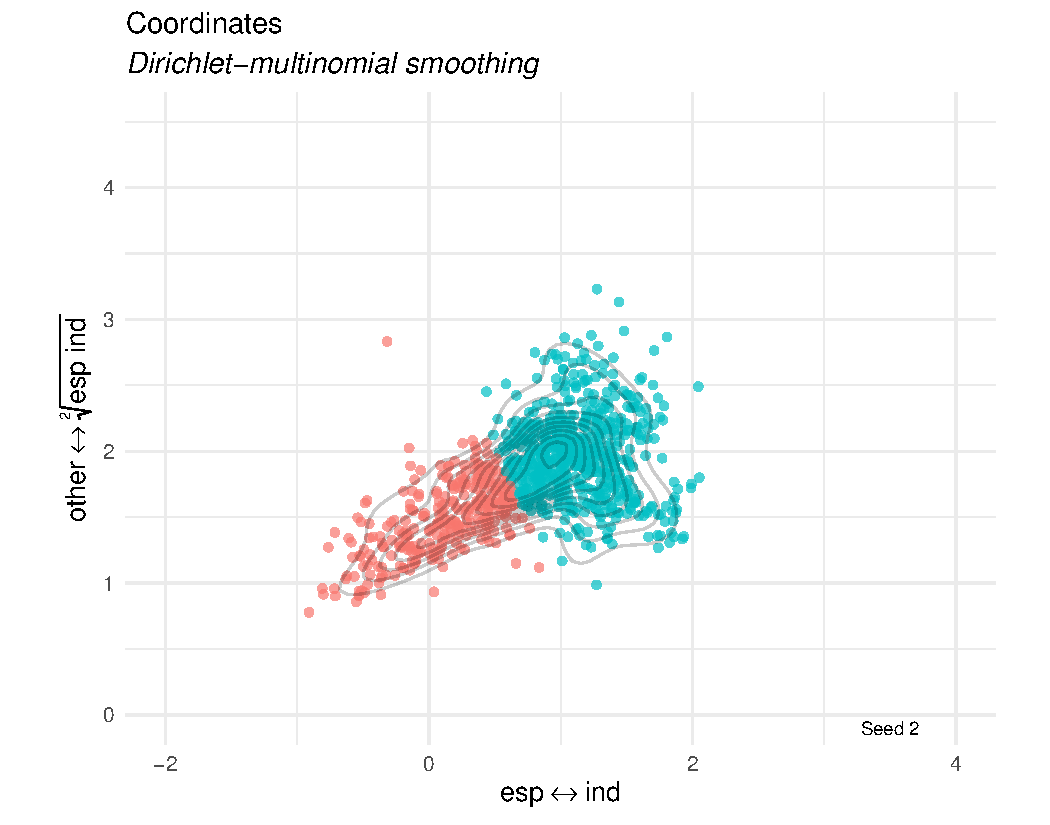
\includegraphics[trim=0cm 0cm 0cm 0cm,width=\textwidth]{sample_cl_nz_2.pdf}}%
\only<6>{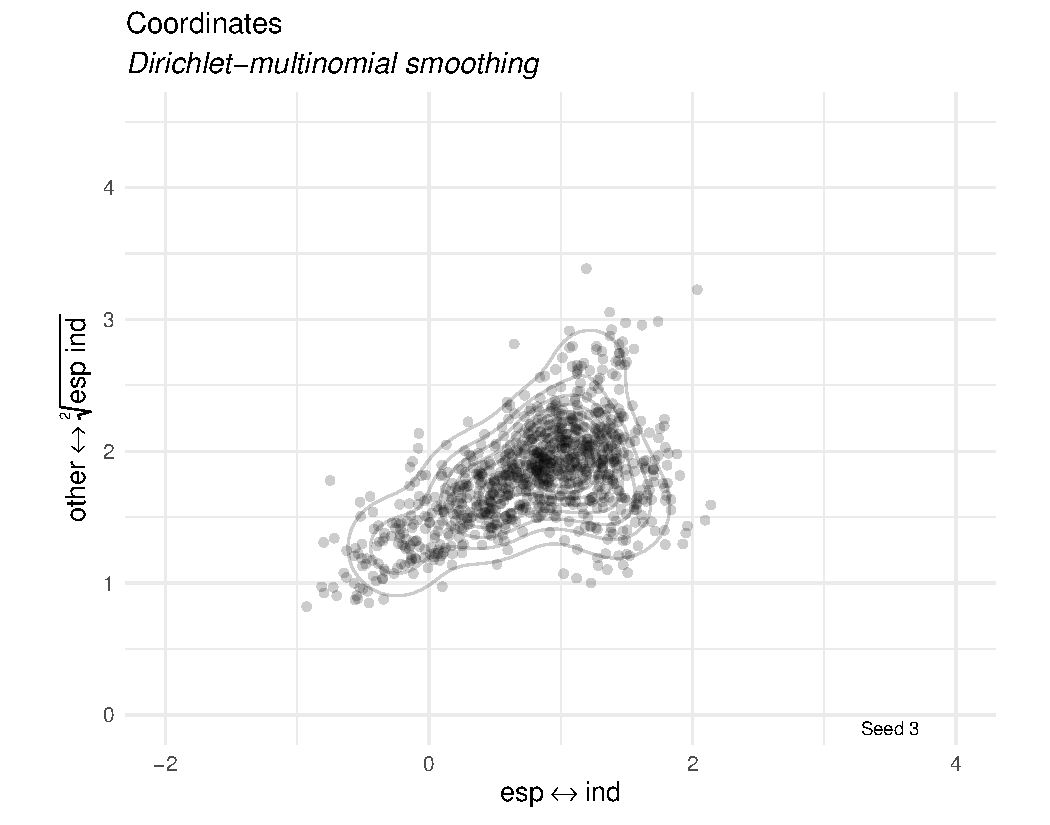
\includegraphics[trim=0cm 0cm 0cm 0cm,width=\textwidth]{sample_nz_3.pdf}}%
\only<7>{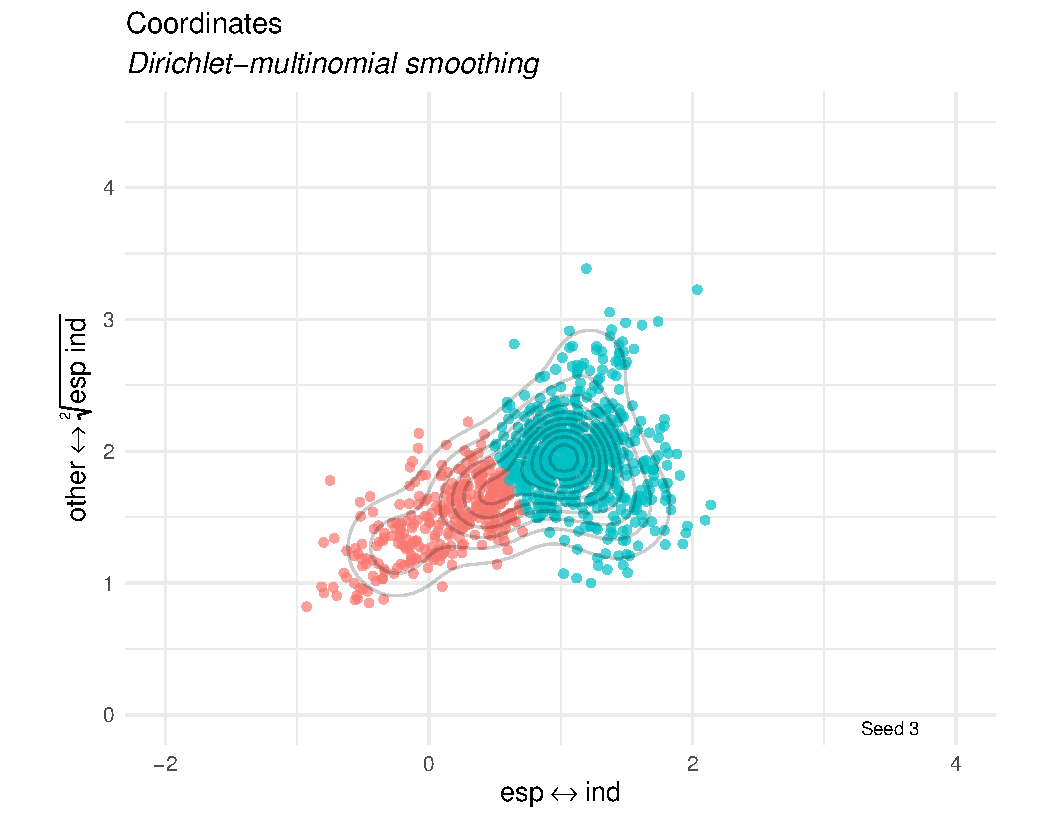
\includegraphics[trim=0cm 0cm 0cm 0cm,width=\textwidth]{sample_cl_nz_3.pdf}}%
\only<8>{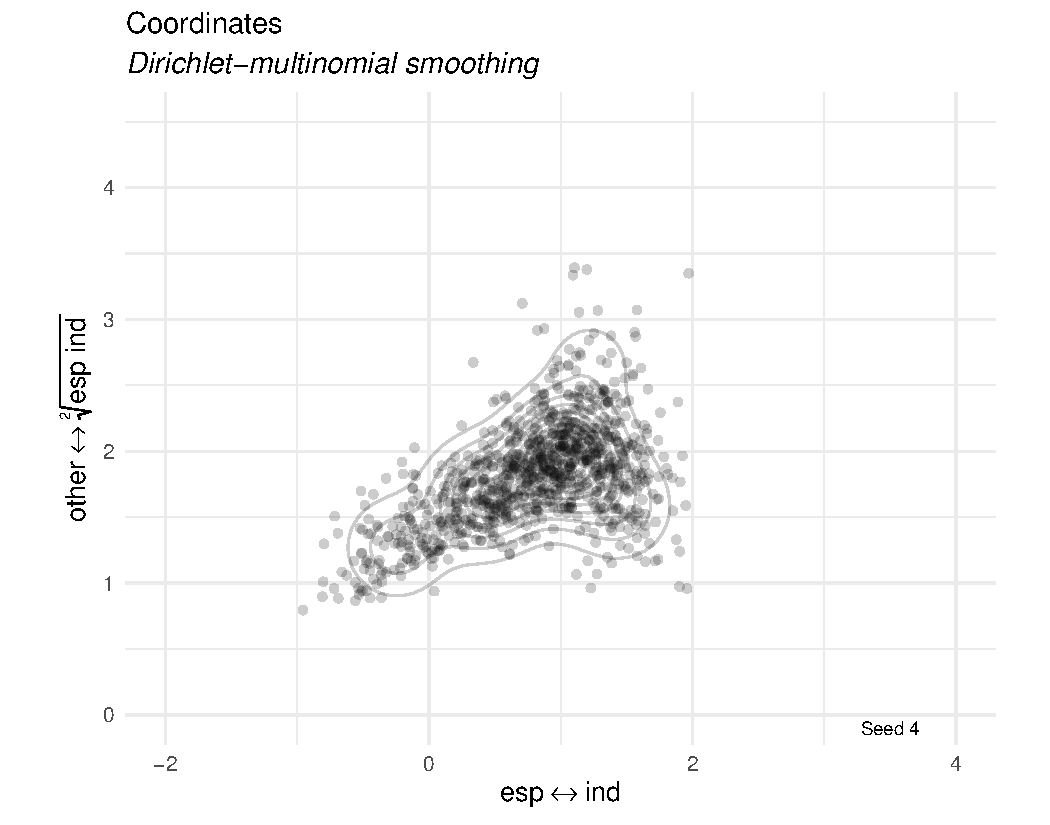
\includegraphics[trim=0cm 0cm 0cm 0cm,width=\textwidth]{sample_nz_4.pdf}}%
\only<9>{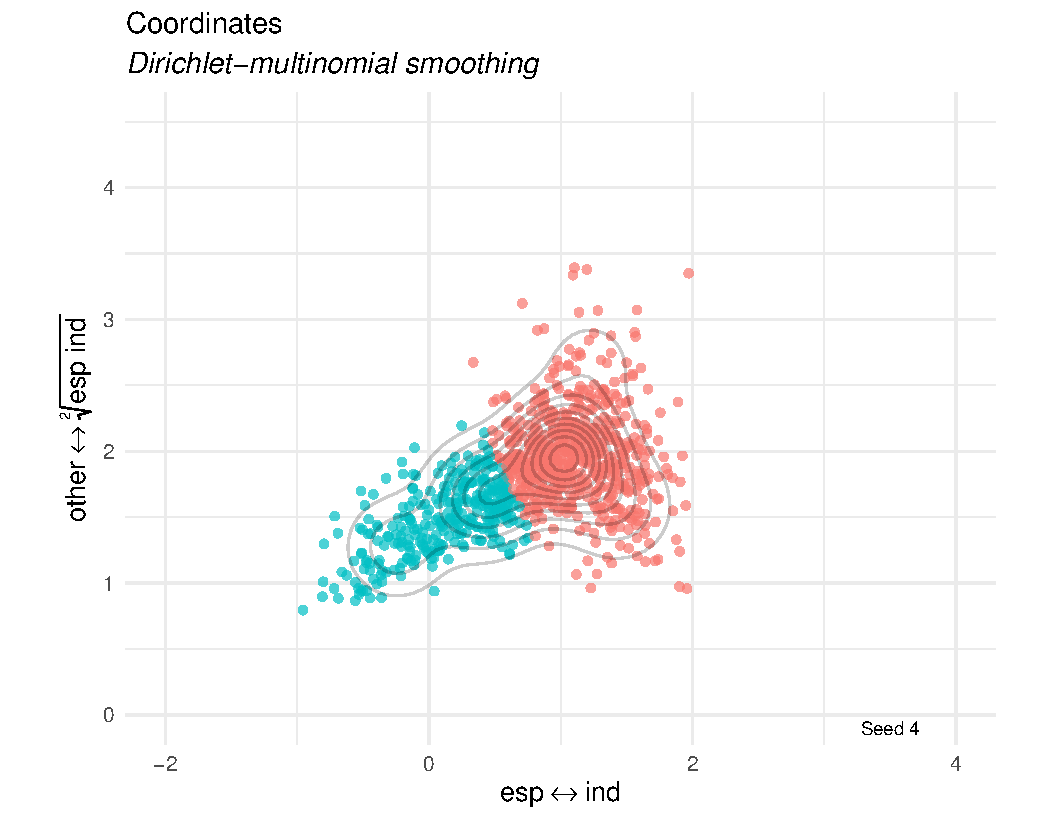
\includegraphics[trim=0cm 0cm 0cm 0cm,width=\textwidth]{sample_cl_nz_4.pdf}}%
\end{figure}
\end{column}
\end{columns}

\vspace{-0.26cm}
\begin{exampleblock}{Creating new samples}
\begin{itemize}
\item[$\rightarrow$]<1-> Using the posterior distribution we can create  $B$  new samples ($B=100$),
\item[$\rightarrow$]<2-> and applying a clustering algorithm ($k$-means, $k\in\{2,\dots,10\}$, Calinski-Harabasz index).
\end{itemize}
\end{exampleblock}

\end{frame}

\begin{frame}[t]{Consensus clustering}

\begin{itemize}
\item Consensus clustering can be applied to summarise all B clusterings. 
\begin{itemize}\item[$\rightarrow$] Majority voting (Dudoit and Fridlyand, 2003)).\end{itemize}
\item<4> Only \emph{four} municipalities differ in the final clustering.
\end{itemize}

\begin{columns}
\begin{column}{0.5\textwidth}
\begin{figure}\vspace{-0.20cm}%
\only<1>{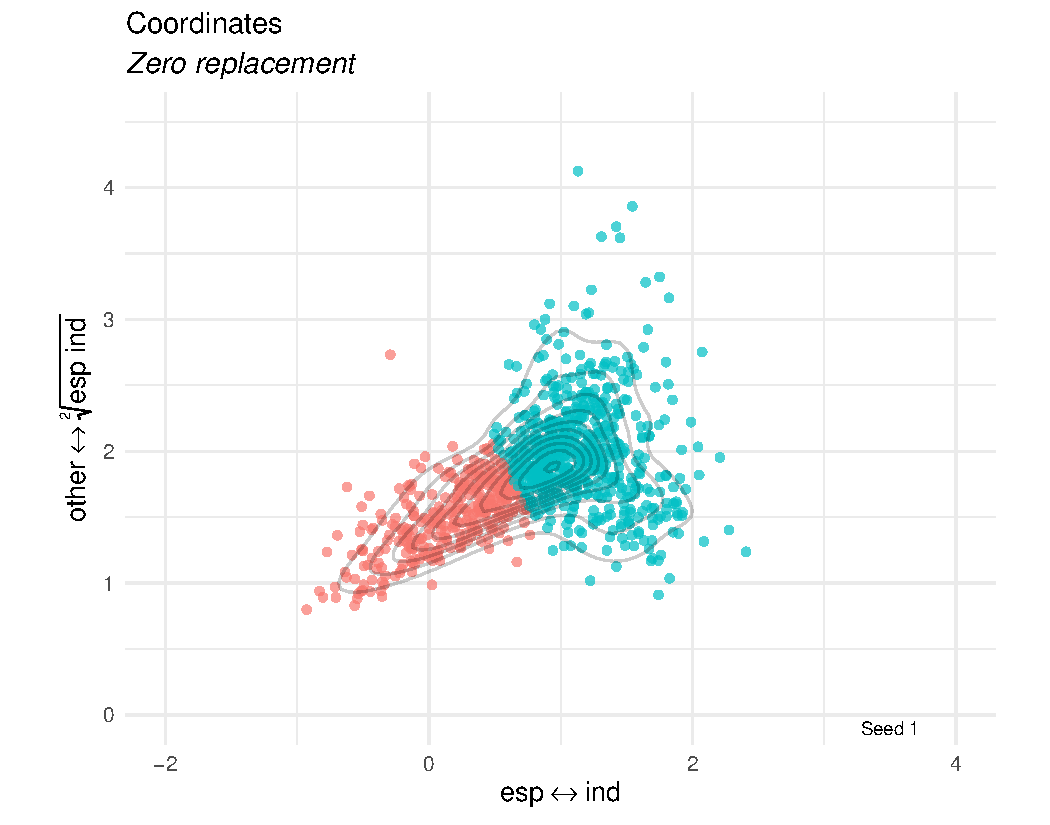
\includegraphics[trim=0cm 0cm 0cm 0cm,width=0.45\textwidth]{sample_cl_zr_1.pdf}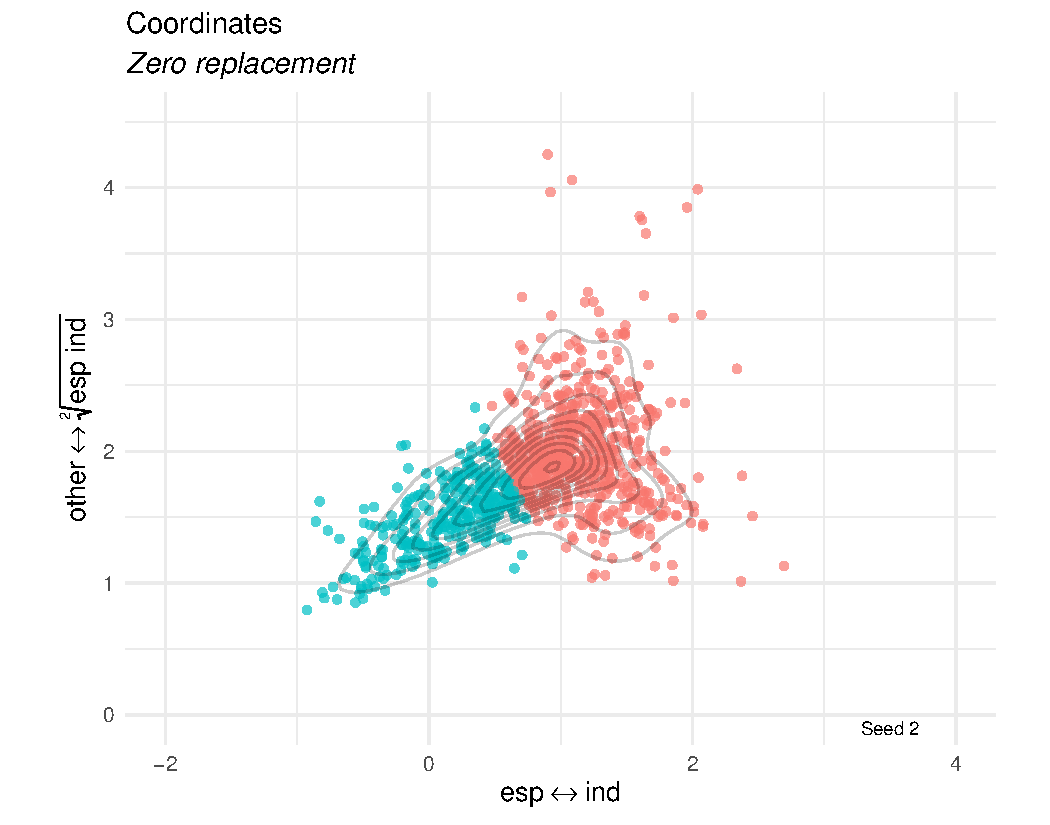
\includegraphics[trim=0cm 0cm 0cm 0cm,width=0.45\textwidth]{sample_cl_zr_2.pdf}\\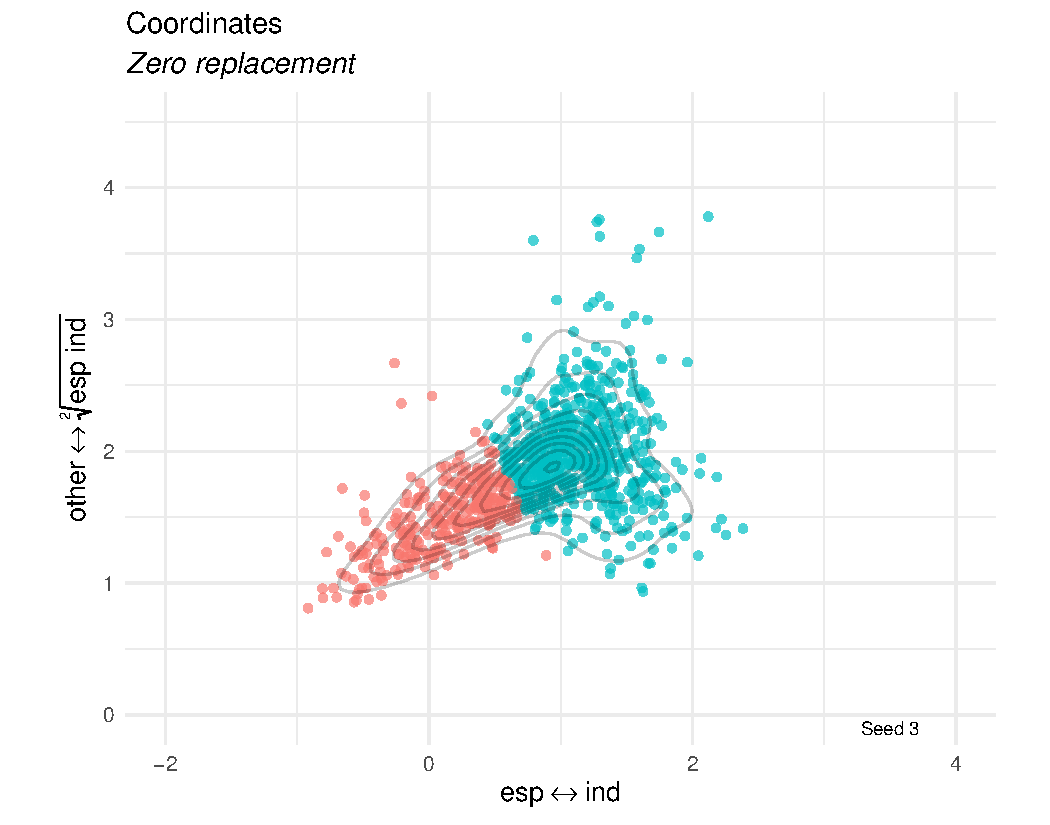
\includegraphics[trim=0cm 0cm 0cm 0cm,width=0.45\textwidth]{sample_cl_zr_3.pdf}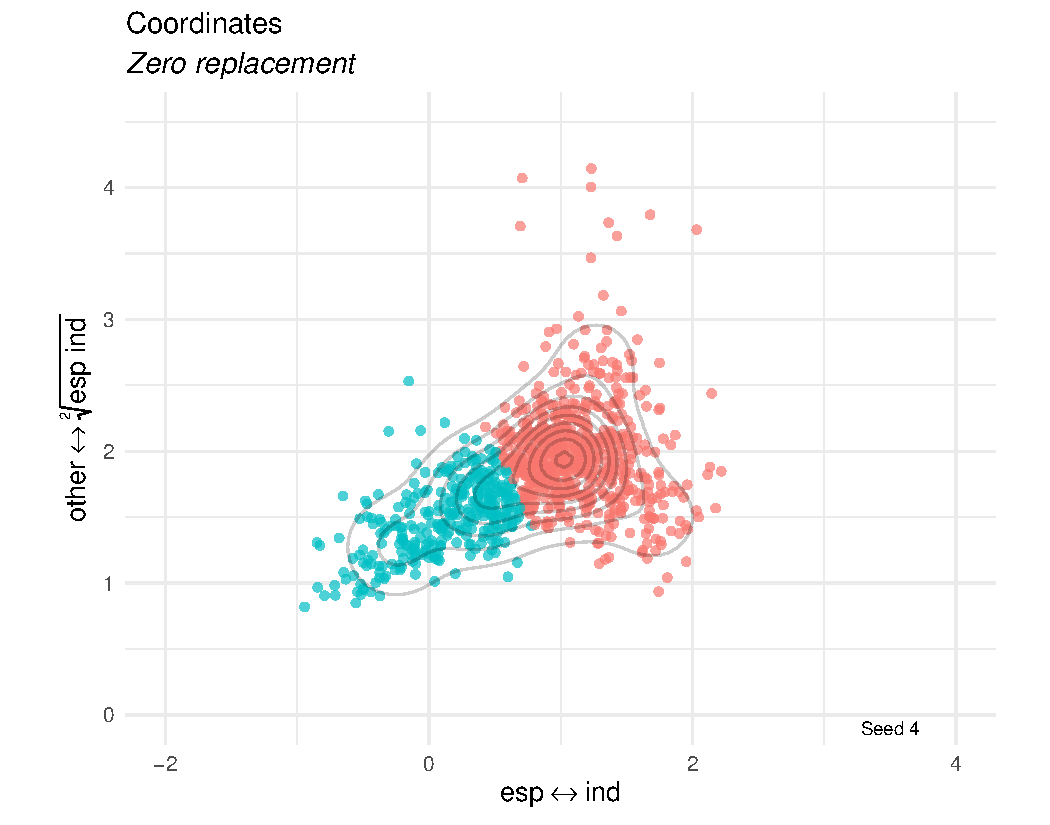
\includegraphics[trim=0cm 0cm 0cm 0cm,width=0.45\textwidth]{sample_cl_zr_4.pdf}}
%\only<10>{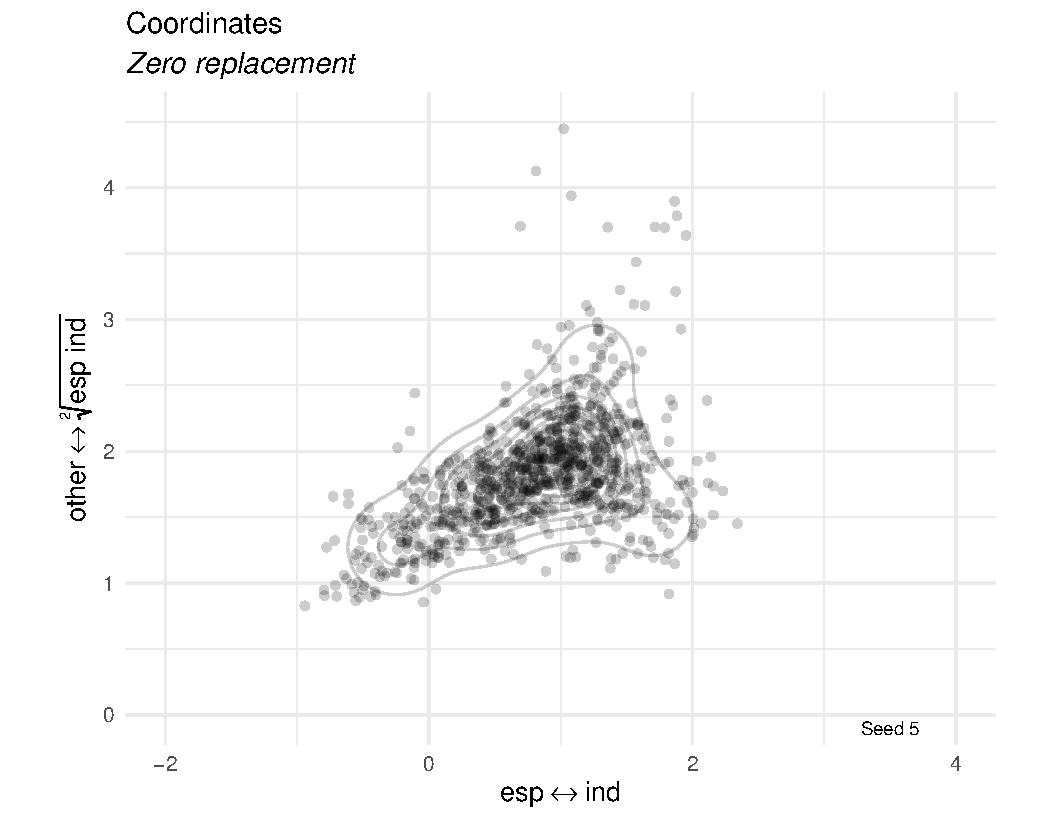
\includegraphics[trim=0cm 0cm 0cm 0cm,width=\textwidth]{sample_zr_5.pdf}}%
%\only<11-12>{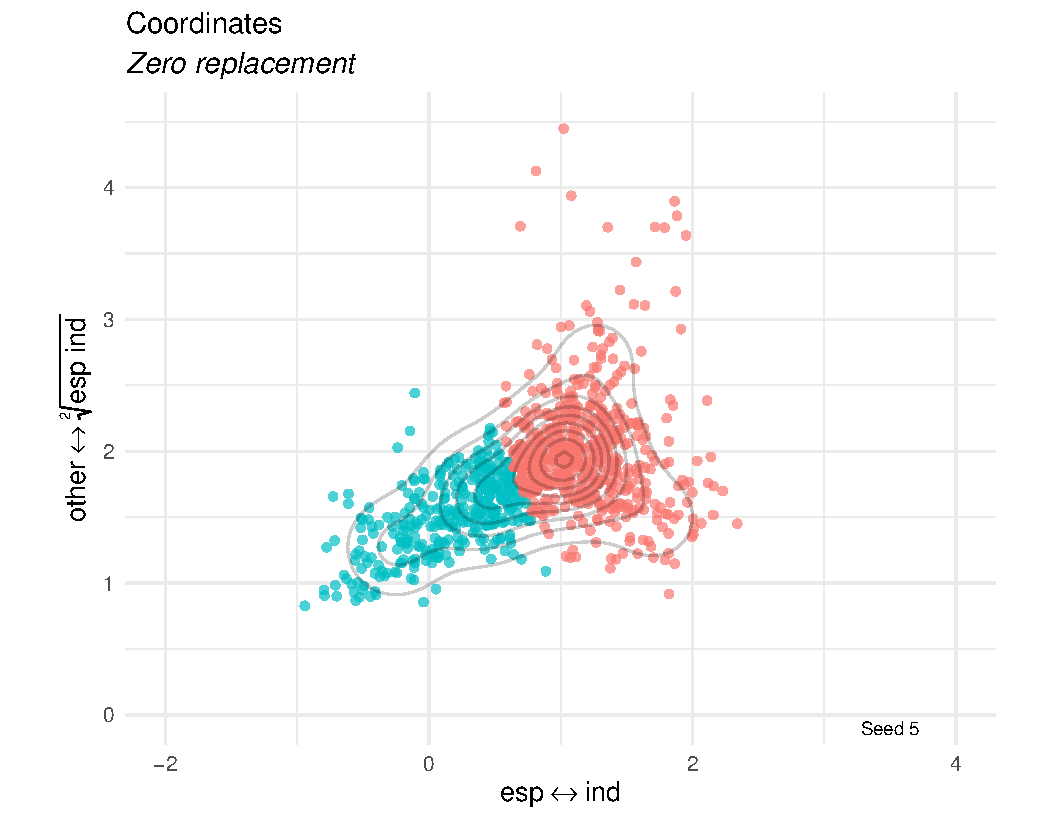
\includegraphics[trim=0cm 0cm 0cm 0cm,width=\textwidth]{sample_cl_zr_5.pdf}}%
\only<2>{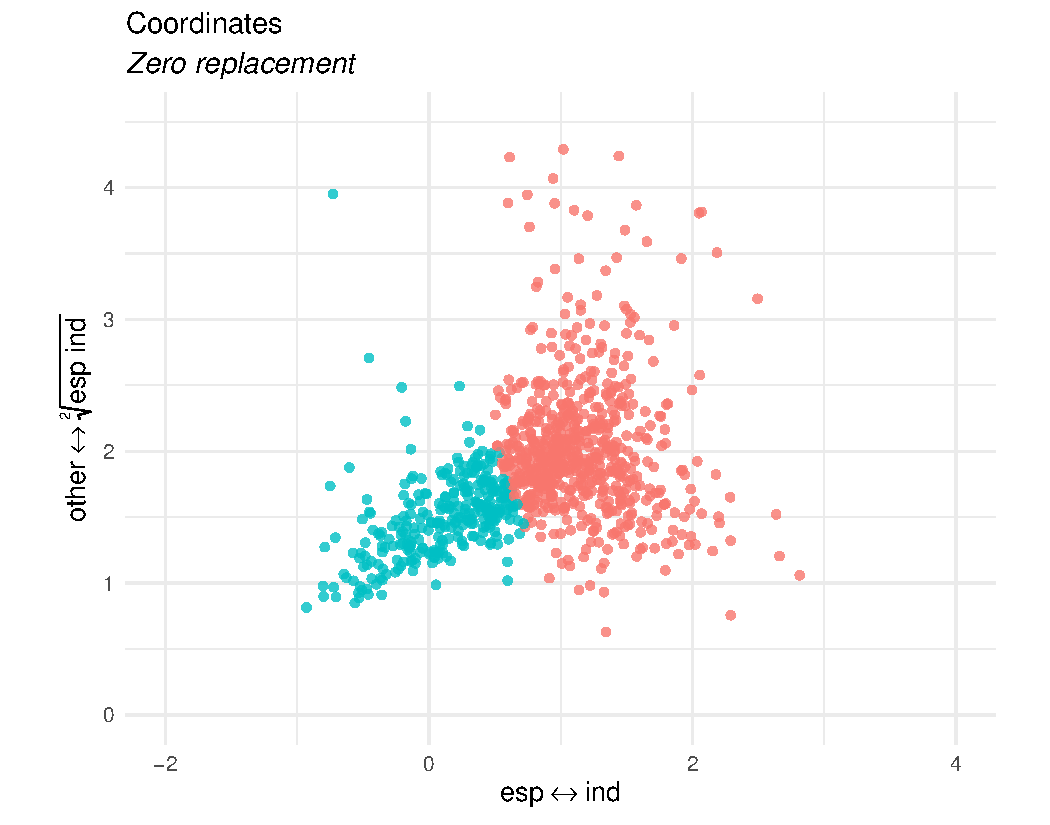
\includegraphics[trim=0cm 0cm 0cm 0cm,width=\textwidth]{clustering_zr.pdf}}%
\only<3>{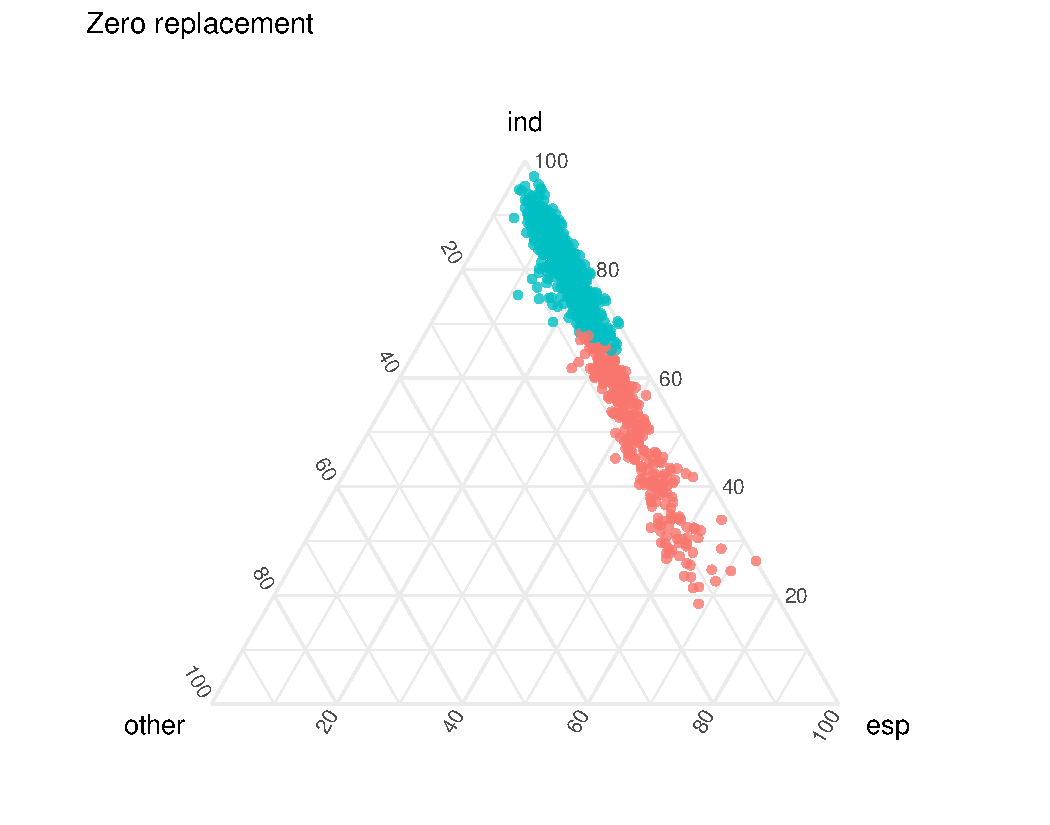
\includegraphics[trim=0cm 0cm 0cm 0cm,width=\textwidth]{clustering_tern_zr.pdf}}%
\only<4>{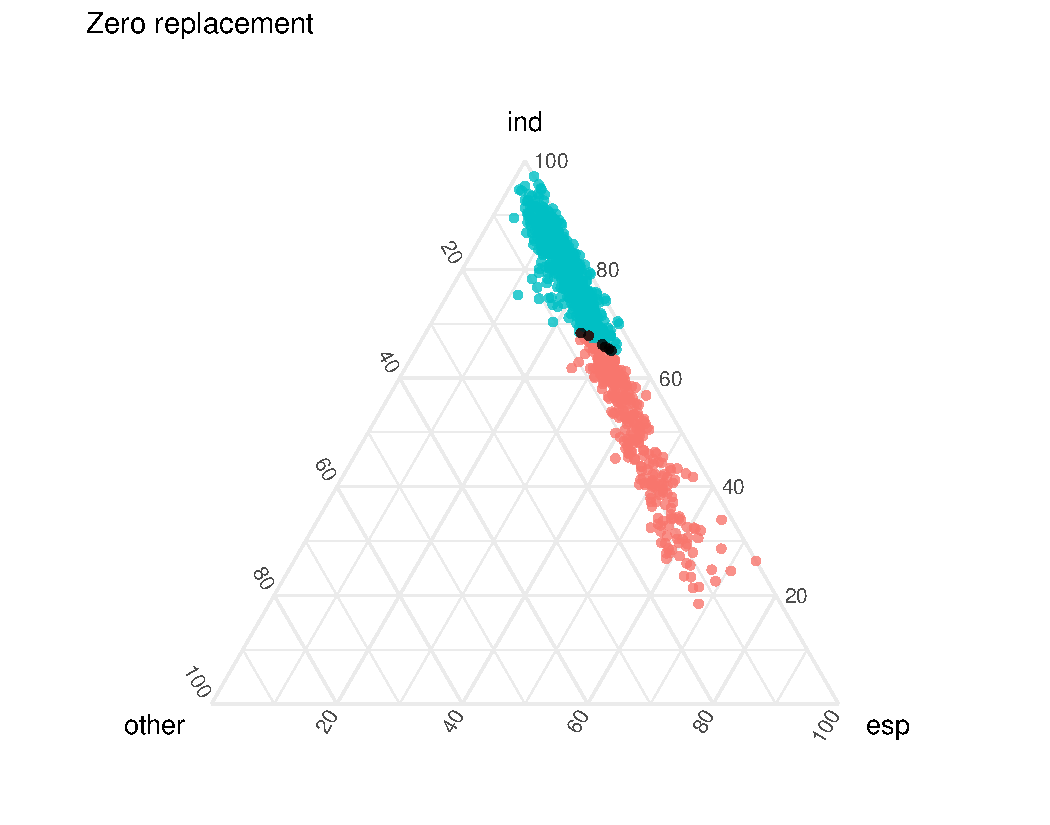
\includegraphics[trim=0cm 0cm 0cm 0cm,width=\textwidth]{clustering_tern_diff_zr.pdf}}%
\end{figure}
\end{column}
\begin{column}{0.5\textwidth}%
\begin{figure}\vspace{-0.20cm}
\only<1>{\includegraphics[trim=0cm 0cm 0cm 0cm,width=0.45\textwidth]{sample_cl_nz_1.pdf}\includegraphics[trim=0cm 0cm 0cm 0cm,width=0.45\textwidth]{sample_cl_nz_2.pdf}\\\includegraphics[trim=0cm 0cm 0cm 0cm,width=0.45\textwidth]{sample_cl_nz_3.pdf}\includegraphics[trim=0cm 0cm 0cm 0cm,width=0.45\textwidth]{sample_cl_nz_4.pdf}}%
%\only<10>{\includegraphics[trim=0cm 0cm 0cm 0cm,width=\textwidth]{sample_nz_5.pdf}}%
%\only<11-12>{\includegraphics[trim=0cm 0cm 0cm 0cm,width=\textwidth]{sample_cl_nz_5.pdf}}%
\only<2>{\includegraphics[trim=0cm 0cm 0cm 0cm,width=\textwidth]{clustering_nz.pdf}}%
\only<3>{\includegraphics[trim=0cm 0cm 0cm 0cm,width=\textwidth]{clustering_tern_nz.pdf}}%
\only<4>{\includegraphics[trim=0cm 0cm 0cm 0cm,width=\textwidth]{clustering_tern_diff_nz.pdf}}%
\end{figure}
\end{column}
\end{columns}

\end{frame}


\begin{frame}{Final remarks}

\begin{itemize}
\item An approach to cluster count data when only the relative relation between parts is of interest has been presented.\vspace{0.2cm}
%\item Methods using compositional covariance (those based on the normality) have very limited applicability. They are computational demanding.\vspace{0.2cm}
\item A parametric approach can be constructed in such a way that the variability coming from a multinomial counting process can be incorporated to the observed compositional variability.\vspace{0.2cm}
\item To obtain a final clustering, consensus clustering algorithms can be applied to clustering obtained  from each sample.
\end{itemize}
\end{frame}






\end{document}
